\chapter{Biometría}\label{apendix:Biometria}

%%%%%%%%%%%%%%%%%%%%%%%% BIOMETRIA Y SISTEMAS BIOMETRICOS    %%%%%%%%%%%%%%%%%%%%%%%%%%%%%%
\section{Biometría y sistemas biométricos}\label{sec:Biometria}

La necesidad de reconocerse entre congéneres es algo común y necesario entre la mayor parte de los animales. Cada especie hace uso de los sentidos que tiene más desarrollados: el tacto, la vista, el oído o el olfato. Pero en el caso de los seres humanos, se dispone además de otros mecanismos que les permiten identificarse.

\begin{itemize}
    \item
    \textbf{Eres lo que posees}: Consiste en identificarse mediante un \textbf{token físico}: un documento, una tarjeta o algún tipo de llave. Puede ser un buen sistema de identificación pero tiene un problema, el objeto que sirve para identificase se \textbf{puede perderse o ser robado}.
    \item
    \textbf{Eres lo que conoces}: Identificarse mediante alguna \textbf{\textit{``santo y seña''}} o alguna \textbf{contraseña} preestablecida. En este caso no existe el problema de perder la identificación, pero se corre el riesgo de \textbf{olvidarla}. 
    \item
    \textbf{Eres lo que eres}: Identificarse por \textbf{características fisiológicas} o de \textbf{comportamiento}, de manera que no se corre el riesgo ni de extraviar una llave, ni de olvidar una contraseña. Esta capacidad de identificarse se basa en la \textbf{\gls{biometria}}.
\end{itemize}

El origen etimológico del termino \gls{biometria} viene derivado de dos palabras griegas: \textit{<<bio>>} (vida) y \textit{<<métron>>} (medida) y se refiere al uso de \textbf{rasgos físicos} o de \textbf{comportamiento} para la \textbf{identificación de individuos}. Físicos como la huella dactilar o los rasgos faciales, y comportamientos como la forma de escribir o la manera de caminar.

El objetivo de la biometría es de encontrar un patrón único que identifique a cada individuo basándose en características físicos o de comportamiento. \cite{li2009encyclopedia}. Este patrón es lo que se conoce como rasgo biométrico.

A la hora de elegir un rasgo biométrico se deben de tener en cuenta los siguientes factores, que sirven para medir la \textbf{calidad del rasgo}: 

\begin{itemize}
    \item
    \textbf{Universalidad}: Todos los individuos que deseen ser identificados deben poseer el rasgo.
    \item
    \textbf{Singularidad}: El rasgo debe tener la capacidad de discriminación suficiente como para permitir diferenciar claramente a un individuo del resto.
    \item
    \textbf{Ponderabilidad}: Debe poder medirse de forma cuantitativa.
    \item
    \textbf{Persistencia} y \textbf{estabilidad}: El rasgo debe conservarse en el tiempo y no perderse por las condiciones ambientales o por factores como una enfermedad o un accidente. Algunos rasgos tienen un periodo de estabilidad corto, lo requiere que se actualice su registro cada cierto tiempo, como por ejemplo, los rasgos faciales).
    \item
    \textbf{Rendimiento} y \textbf{calidad}: Que el rasgo permita extraer datos claros, precisos y fácilmente analizables sin necesidad de costosos preprocesos.
    \textbf{Usabilidad}: El rasgo debe ser fácilmente adquirido incluso en personas con alguna restricción física o alguna discapacidad.
    \item
    \textbf{Vulnerabilidad}: El rasgo debe ser resistente frente a ataques, debe ser resistente frente a suplantaciones u ocultaciones.
    \item
    \textbf{Privacidad}: El acceso al rasgo biométrico debe ser lo más restringido posible y si es necesario almacenarlo debe ser posible encriptarlo.
    \item
    \textbf{Aceptación}: La adquisición del rasgo debe ser consentida por el individuo y no suponer un agravio sea cual se su cultura o creencias.   
    \item
    \textbf{Escalabilidad}: Los procesos necesarios para la identificación deben ser rápidos, especialmente, en sistemas con gran número de usuarios.
    \item
    \textbf{Mantenimiento}: Es deseable que los sensores no requieran demasiados cuidados de limpieza o que sufran un desgaste excesivo. 
    \item
    \textbf{Integración}: Que sea posible compatibilizar la identificación biométrica con otro tipo de identificación.
\end{itemize}


%%%%%%%%%%%%%%%%%%%%%%%%%%%%%%%%%%%% BIOMETRIA:SISTEMAS BIOMÉTRICOS %%%%%%%%%%%%%%%%%%%%%%
\section{Sistemas biométricos}\label{sec:SistemasBiometricos}

La verificación de la identidad mediante la biometría también se conoce como \textbf{identificación biométrica} \cite{li2009encyclopedia}. Los sistemas encargados de la identificación biométrica se conocen como \textbf{sistemas biométricos} y la mayoría de ellos están relacionadas con la seguridad..

% \color{red}
% En general los sistemas biométricos buscan mejorar la calidad de vida de las personas pero, antes de implantar un sistema biométrico se deben evaluar, los costes que conlleva (sensores, equipos, etc.) frente a los costes que ahorra (recursos humanos, perdidas de tarjetas etc.).

% La investigación en sensores biométricos comenzó en los años $60$ y ya en $70$ aparecieron los primeros sistemas automáticos que usaban la biometría.

% Actualmente los sistemas biométricos automáticos se han extendido a múltiples aplicaciones cada vez mejores cotas de aceptación y de seguridad.

% Una de las razones por las que la \gls{biometria} se ha extendido es por que resulta fácil y rápido.

% Reduce los costes y que no requiere tanta supervisión.
% \color{black}

Los sistemas biométricos se componen de dos etapas o procesos: \textbf{adquisición} y \textbf{verificación} y como el rendimiento del proceso de verificación depende de la calidad del rasgo biométrico adquirido, algunos sistemas incluyen otro módulo que evalúa la \textbf{calidad del rasgo}. Preferiblemente, para una mayor flexibilidad, cada proceso debe estar implementado en un módulo diferente, de forma que sea posible modificar un módulo sin tener que cambiar el sistema completo.

Dependiendo del módulo que que guíe la identificación se distinguen dos tipos de sistemas:
\begin{itemize}
    \item
    Sistemas biométricos \textbf{guiados por la calidad}:
    \item
    sistemas biométricos \textbf{guiados por el \textit{score} de verificación}:
\end{itemize}

Una parte fundamental de un sistema biométrico es el proceso de adquisición o \gls{captura}. Los factores a tener en cuenta para realizar una buena adquisición son:
\begin{itemize}
    \item 
    Disponer de bueno dispositivos de adquisición que permitan capturar de forma correcta toda la información que posteriormente se necesitará en la verificación o en la identificación.
    \item
    Tener en cuenta factores de \gls{ergonomia} que faciliten la \gls{captura}. Por ejemplo, usar varias cámaras para la \gls{captura} \gls{facial} o permitir que la lectura de ambas manos en la biometría dactilar o de la palma de la mano.
    \item
    Controlar, en la medida de lo posible las condiciones ambientales. Por ejemplo, la iluminación o el fondo a la hora de realizar una \gls{captura} facial o la humedad y la suciedad en el lector para las huellas dactilares.
    \item
    Conviene tener en cuenta la \gls{usabilidad} del sistema y sobretodo, la señalización y la información suministrada al usuario para que éste tenga claras las instrucciones que debe seguir. Por ejemplo, que pose tomar, que expresiones evitar o como presionar el sensor de huellas.
    \item
    otra buena practica es, implementar algoritmos de control de calidad para controlen que la \gls{captura} se ha realizado correctamente.
    \item
    El uso de \gls{multi-biometria} también puede solucionar problemas de adquisición ya que al capturar varios rasgos, es más probable que alguno de ellos esté correctamente capturado \cite{jain2007handbook} \cite{snelick2003multimodal} \cite{jain2004multibiometric}.  
\end{itemize}


%%%%%%%%%%%%%%%%%%%%%%%%%%%%%%%%%%%% BIOMETRIA:FASES DE UN SITEMA BIOMETRICO %%%%%%%%%%%%%%%%%%%%%%%%%%%
\section{Módulos de un sistema biométrico}\label{sec:ModulosSistemasBiometricos}

\begin{figure}[t]
    \centering
    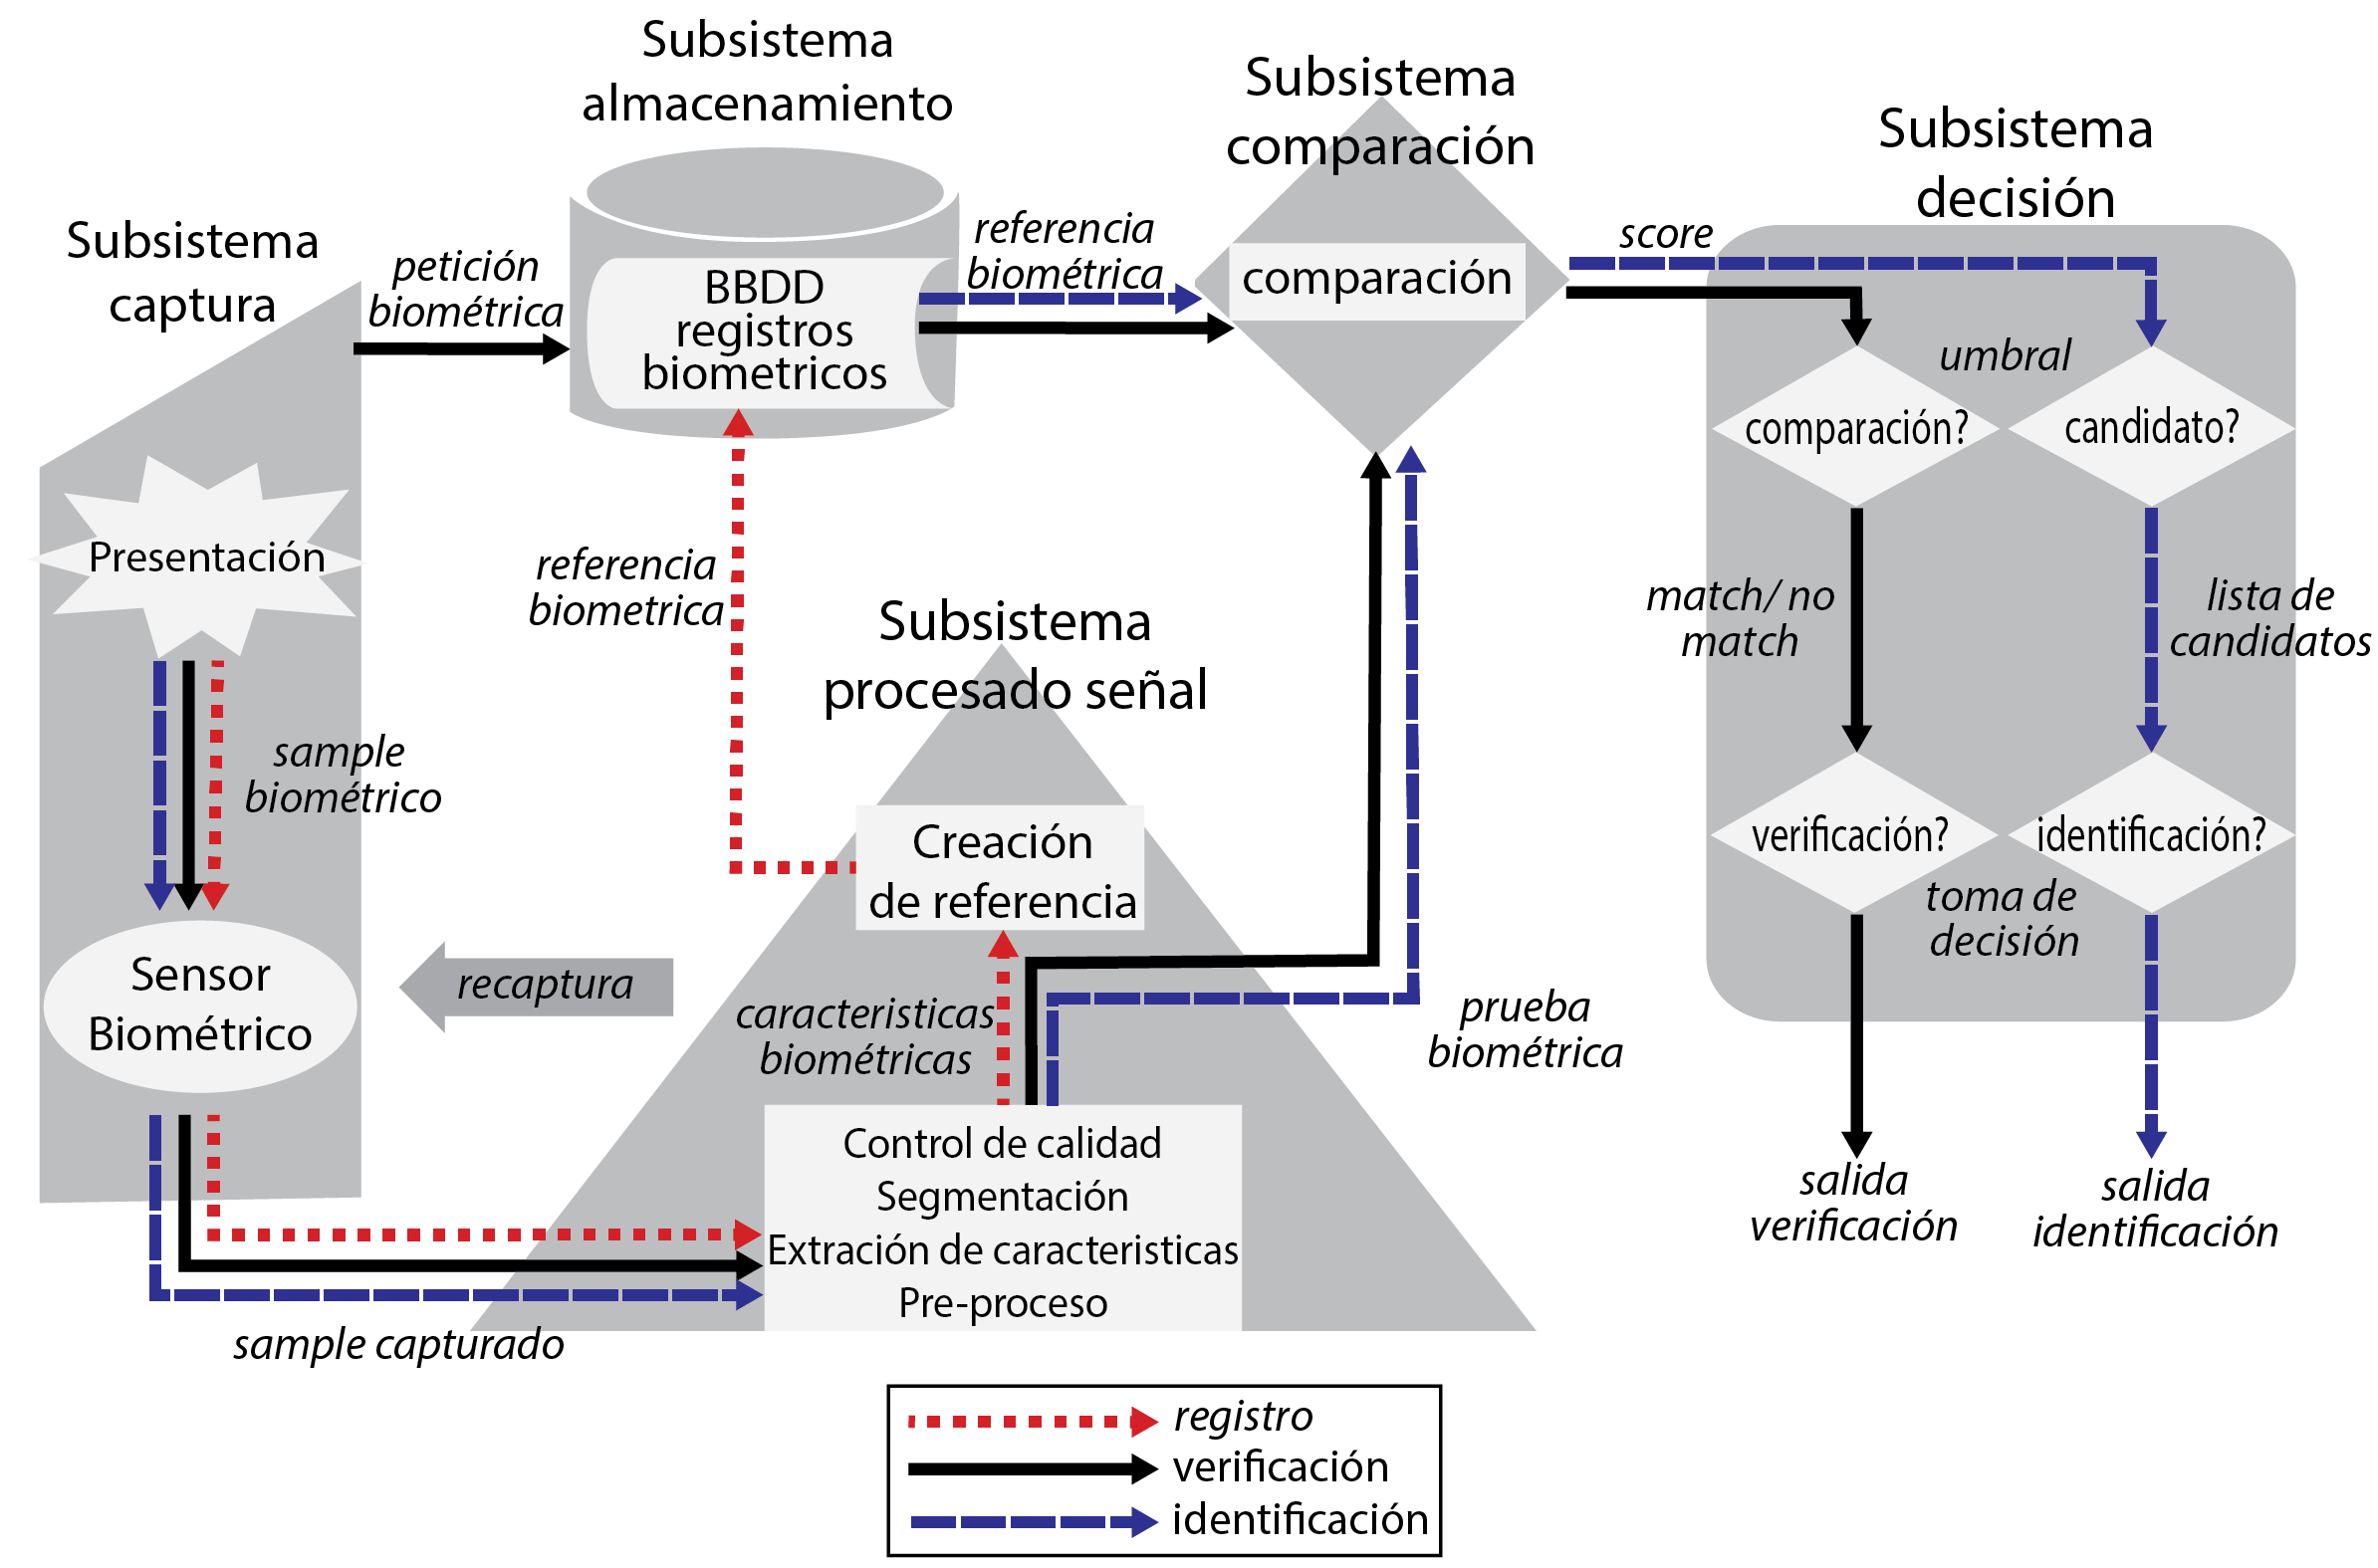
\includegraphics[width=0.8\textwidth]{ch-sistemasABC/images/ch-sistemasBiometricos/esquemaSistemaBiometricos.png}
    \caption{Esquema sistema biométrico \cite{ISO/Biometric}}
    \label{fig:esquemaSistemaBiometrico}
\end{figure}

Los sistemas biométricos usan la biometría para \textbf{autenticar a usuarios registrados} en el sistema. En la figura \ref{fig:esquemaSistemaBiometrico} se puede ver la arquitectura básica de un sistemas biométrico propuesta por en \GLS{ISO}/\GLS{IEC} JTC$1$ SC$37$, que se compone a su vez de varios subsistemas: captura o adquisición, procesado de la señal, almacenamiento, comparación o \textit{matching} y toma de decisión.

\begin{itemize}
    \item 
    \textbf{Subsistema de captura}:
    
    Recoge la \textbf{información biométrica} de los individuos mediante un sensor.
    \item 
    \textbf{Subsistema de procesado de la señal}:
    
    Procesa la información capturada y extrae las \textbf{características biométricas} que describen de forma univoca al individuo.  
    
    Se no es posible procesar el rasgo o extraer las características, el sistemas puede proceder a una \textbf{recaptura} del rasgo.
    \item 
    \textbf{Subsistema de almacenamiento}:
    
    Repositorio que almacena las \textbf{plantillas de referencia} construidas con las características del individuo. Cada usuario del sistema debe tener una plantilla de referencia con sus características biométricas, registrada en el subsistema de almacenamiento. 
    \item 
    \textbf{Subsistema de comparación}:
    
    Permite obtener un \textbf{\textit{score} o puntuación de semejanza} entre las características biométricas extraídas del individuo a autenticar y las características de una plantilla de referencia de subsistema de almacenamiento.
    
    El \textit{score} de semejanza normalmente, es un valor en el rango [$0$,$1$], más cercano a $1$ cuanto más se parezcan las características del individuo a las características de la plantilla registrada.
    
    \item 
    \textbf{Subsistema de decisión}:
    
    El resultado final de un sistema biométrico debe ser un \textbf{\textit{matching-pair}} o un \textbf{\textit{non-matching-pair}}. O lo que es lo mismo, una \textbf{aceptación} o un\textbf{rechazo} de individuo. El subsistema de decisión determinará un resultado u otro, atendiendo a un \textbf{umbral de semejanza}. Si el \textit{score} de semejanza de la comparación, es mayor o igual que el umbral, el resultado será un \textit{matching-pair} y el usuario será aceptado, mientras que si es menor, el resultado será un \textit{non-matching-pair} y el usuario será rechazado.
\end{itemize}

Los sistemas biométricos tienen dos fases: el \textbf{registro} y la \textbf{autenticación}, y cada una de ellas define un proceso diferente. Además el proceso de autenticación puede tratarse de un proceso de identificación o un proceso de verificación.

\begin{itemize}
    \item 
    \textbf{Registro}:
    Es el proceso de inscribir a un individuo como \textbf{usuario del sistema} y consiste en: Capturar los \textbf{datos biométricos} del individuo, construir un \textbf{plantilla de referencia} con las características extraídas de los datos y almacenar dicha plantilla en el \textbf{subsistema de almacenamiento}. 
    \item 
    \textbf{Autenticación}:
    Es el proceso de compro abar si un individuo es un usuario registrado del sistema. Este proceso puede ser una verificación o una identificación. \textbf{Verificación} cuando se busca saber si el individuo es un \textbf{usuario determinado} del sistema y \textbf{identificación} cuando se busca saber si el individuo es alguno de los usuarios del sistema \textbf{sin importar quien}. 
    
    Los primeros pasos de una verificación y de una identificación, son los mismos: Capturar los datos biométricos del individuo y extraer sus características. La diferencia radica en el subsistema de comparación y en el subsistema de decisión. En una verificación la comparación se realiza $1$:$1$ con la plantilla de referencia de un \textbf{usuario especifico} del sistema, mientras que en la identificación la comparación es $1$:n con las plantillas de todos los usuarios registrados o al menos, con un \textbf{conjunto de candidatos}. El subsistema de decisión en el caso de la identificación será aceptación cuando al menos una de las comparaciones supere el umbral de semejanza fijado. 
\end{itemize}



%%%%%%%%%%%%%%%%%%%%%%%%%%%%%%%%%%%% BIOMETRIA:ERRORES EN LOS SISTEMAS BIOMÉTRICOS %%%%%%%%%%%%%%%%%%%%%%
\section{Errores en sistemas biométricos}\label{sec:ErroresSistemasBiometricos}   
   
Los sistemas biométricos pueden tener distintos tipos de errores en sus subsistemas\footnote{\GLS{ISO}/\GLS{IEC} $19795$-$2$:$2017$ \cite{ISO/BiometricErrors} describe los errores que puede sufrir un sistema biométrico en sus diferentes componentes.}:

\begin{itemize}
    \item 
    \textbf{Errores en la captura}:
    
    En el subsistema de captura se pueden producir dos tipos de errores: \textit{Failure to Detect} (\textbf{\GLS{FTD}}) o \textit{Failure to Capture} (\textbf{\GLS{FTC}}). Que pueden venir producidos por distintas \textbf{causas}:
    \begin{itemize}
    \item 
    \textbf{Distorsiones}: El mal uso del sensor o una mala pose del individuo pueden producir que el rasgo se deforme de forma no pueda ser localizado. 
    \item 
    \textbf{Oclusiones}: El rasgo biométrico puede quedar parcial o totalmente oculto por suciedad en el sensor, por prendas de vestir o por la propia pose del individuo.
    \item 
    \textbf{Ergonómicos} o de \textbf{usabilidad}: Algún tipo de lesión puede impedir la adquisición del rasgo o directamente, personas con alguna discapacidad o con problemas movilidad no pueden acceder al sensor. 
    \item 
    Condiciones del \textbf{entorno}: Algunas condiciones ambientales, como la iluminación o el ruido, pueden impedir la adquisición de determinados rasgos. 
    \end{itemize}
    
    \item 
    \textbf{Errores en la extracción de características}:
    
    Se conocen como \textit{Failure to Process} (\textbf{\GLS{FTP}}) y se producen cuando se ha realizado una captura de poca calidad que no permite extraer las características del rasgo. Estos errores están muy relacionados con los errores que se producen en el subsistema de captura por eso a los errores \GLS{FTD}, \GLS{FTC} y \GLS{FTP} se le conoce también como \textit{failure to Acquire} (\textbf{\GLS{FTA}}).
    
    Este tipo de errores producen que el resto de los subsistemas no puedan realizar sus procesos correctamente. Una manera de minimizarlos consiste en implementar métodos para evaluar la \textbf{calidad de la captura}. 
    
    \item 
    \textbf{Errores en la construcción de plantillas}:
    
    Cuando se produce una captura de mala calidad o se extraen características de forma errónea, es posible que se produzcan fallos al construir la plantilla de referencia del usuario. Estos errores se conocen como \textit{Failure to Enroll} (\textbf{\GLS{FTE}}). Si no se controlan estos errores el sistema puede registrar \textbf{plantillas incorrectas} difíciles de detectar posteriormente, y que afectarán al subsistema de comparación y al rendimiento general del sistema.  
    
    \item 
    \textbf{Errores en la comparación o en la decisión}:
    
    Como se explica en el punto \ref{sec:ModulosSistemasBiometricos}, el subsistema de decisión debe terminar considerando al usuario como aceptado o como rechazado, atendiendo al \textit{score} obtenido en la comparación. Por eso, un error en la comparación o en la decisión, sucede cuando el resultado final es una \textbf{falsa aceptación} o un \textbf{falso rechazo}. Este tipo de errores se usan para evaluar el rendimiento general del sistema y se describen en profundidad en el punto \ref{sec:MetricasYEvaluacionSistemasbiometricos}.
\end{itemize}


%%%%%%%%%%%%%%%%%%%%%%%%%%%%%%%%%%%% BIOMETRIA:EVALUACION DE SISTEMAS BIOMÉTRICOS %%%%%%%%%%%%%%%%%%%%%%
\section{Métricas y evaluación en sistemas biométricos}\label{sec:MetricasYEvaluacionSistemasbiometricos}

El modulo de decisión pude cometer dos tipos de errores: errores de \textbf{\textit{false match}} o \textbf{falsa aceptación} cuando un individuo no registrado en el sistema (impostor) es aceptado como un usuario valido del sistema, o errores de \textbf{\textit{false non-match}} o de \textbf{falso rechazo} cuando un individuo es un usuario registrado del sistema (genuino) es rechazado.

Para evaluar la precisión de un sistema se requieren un gran número de comparaciones de usuarios registrados con plantillas de referencia correctas, lo que permite obtener \textbf{\textit{genuine distribution}} (la distribución de los \textit{scores} de similitud para comparaciones genuinas). Y también un gran número de comparaciones de usuarios con plantillas de referencia que no les corresponde, para obtener \textbf{\textit{impostor distribution}} (la distribución de los \textit{scores} de similitud para comparaciones no genuinas).  

\textbf{\textit{False Aceptation Rate}} (\textbf{\GLS{FAR}} o \textit{fase match rate} (\GLS{FMR})) es la probabilidad de que se produzca un error de falsa aceptación en el sistema mientras que \textbf{\textit{False Reject Rate}} (\textbf{\GLS{FRR}} o \textit{fase non-match rate} (\GLS{FNMR})) es la probabilidad de que se produzca un error de falso rechazo en un sistema. Como las falsas aceptaciones y los falsos rechazos depende del \textbf{umbral de semejanza t}, el \textbf{\GLS{FAR}(t)} a el \textbf{\GLS{FRR}(t)} también dependen del umbral (ver Figura \ref{fig:distribucionesGenuinoImpostor}).

\begin{figure}[t]
    \centering
    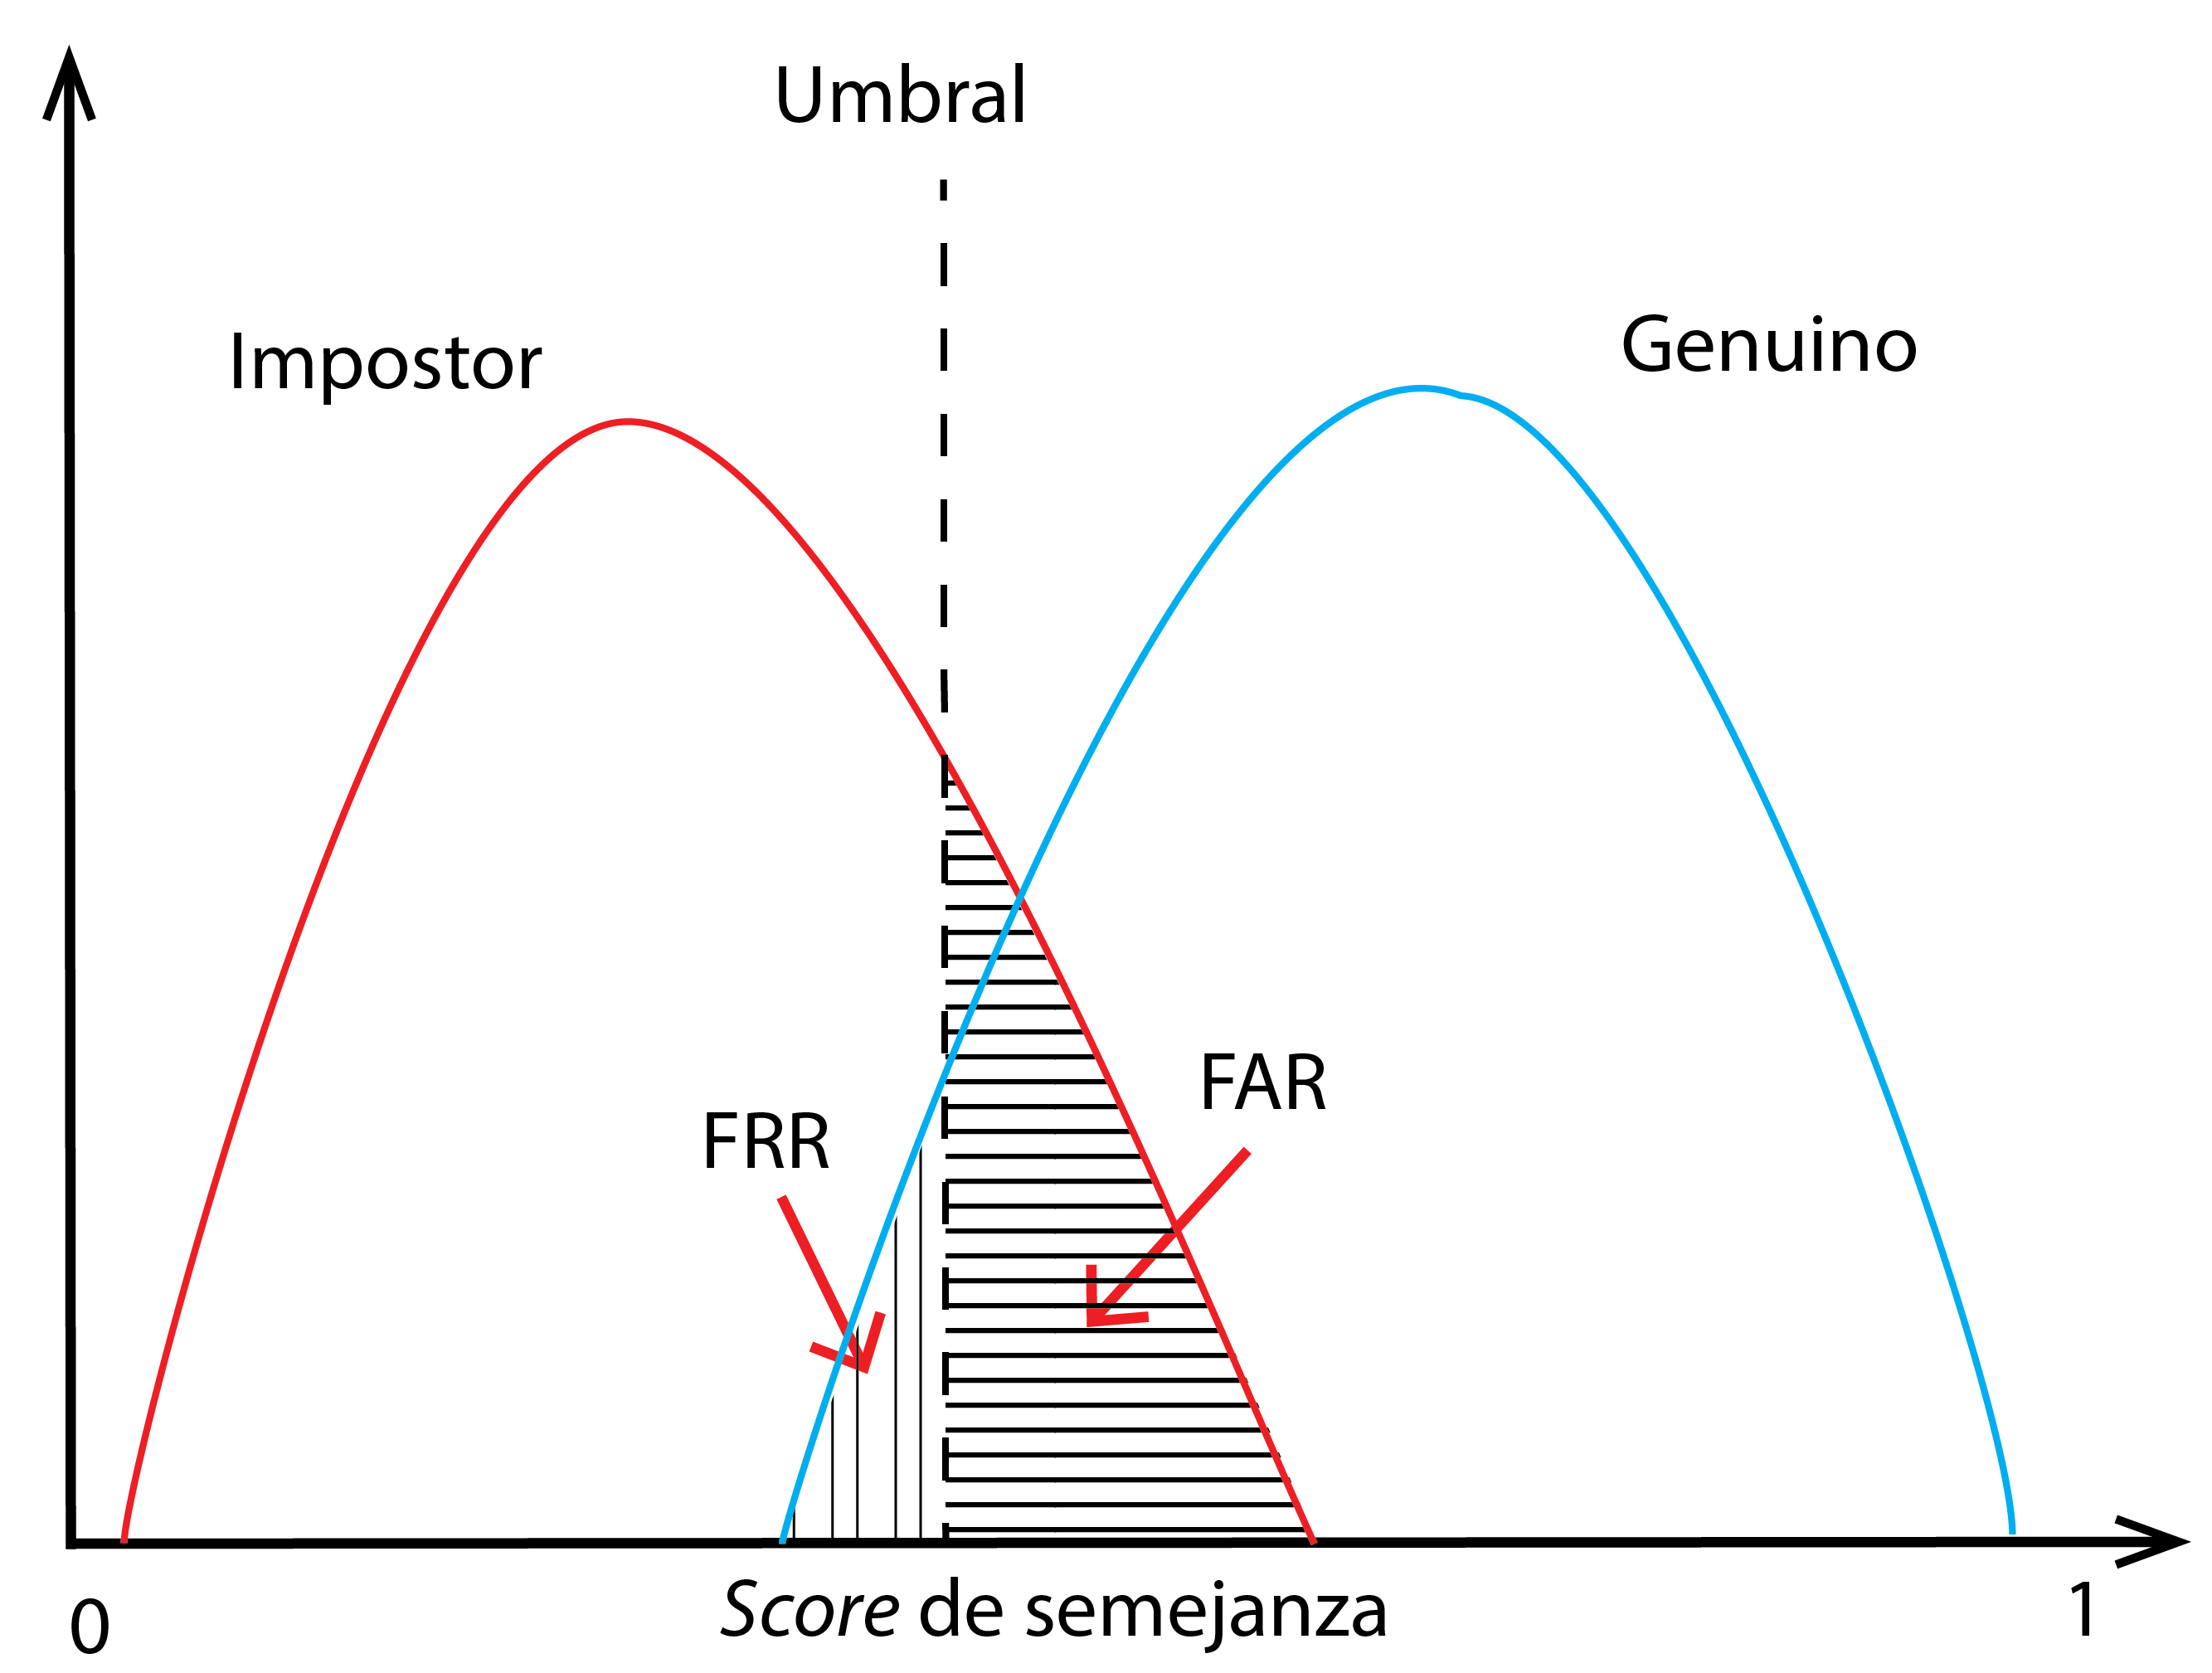
\includegraphics[width=0.5\textwidth]{ch-sistemasABC/images/ch-sistemasBiometricos/curves_DistribucionGenuinoImpostor-01.png}
    \caption{Distribución de genuinos e impostores con errores \textit{False Reject Rate} (\GLS{FRR}) y \textit{False Accept Rate} (\GLS{FAR})}
    \label{fig:distribucionesGenuinoImpostor}
\end{figure}

\begin{figure}[t]
    \centering
    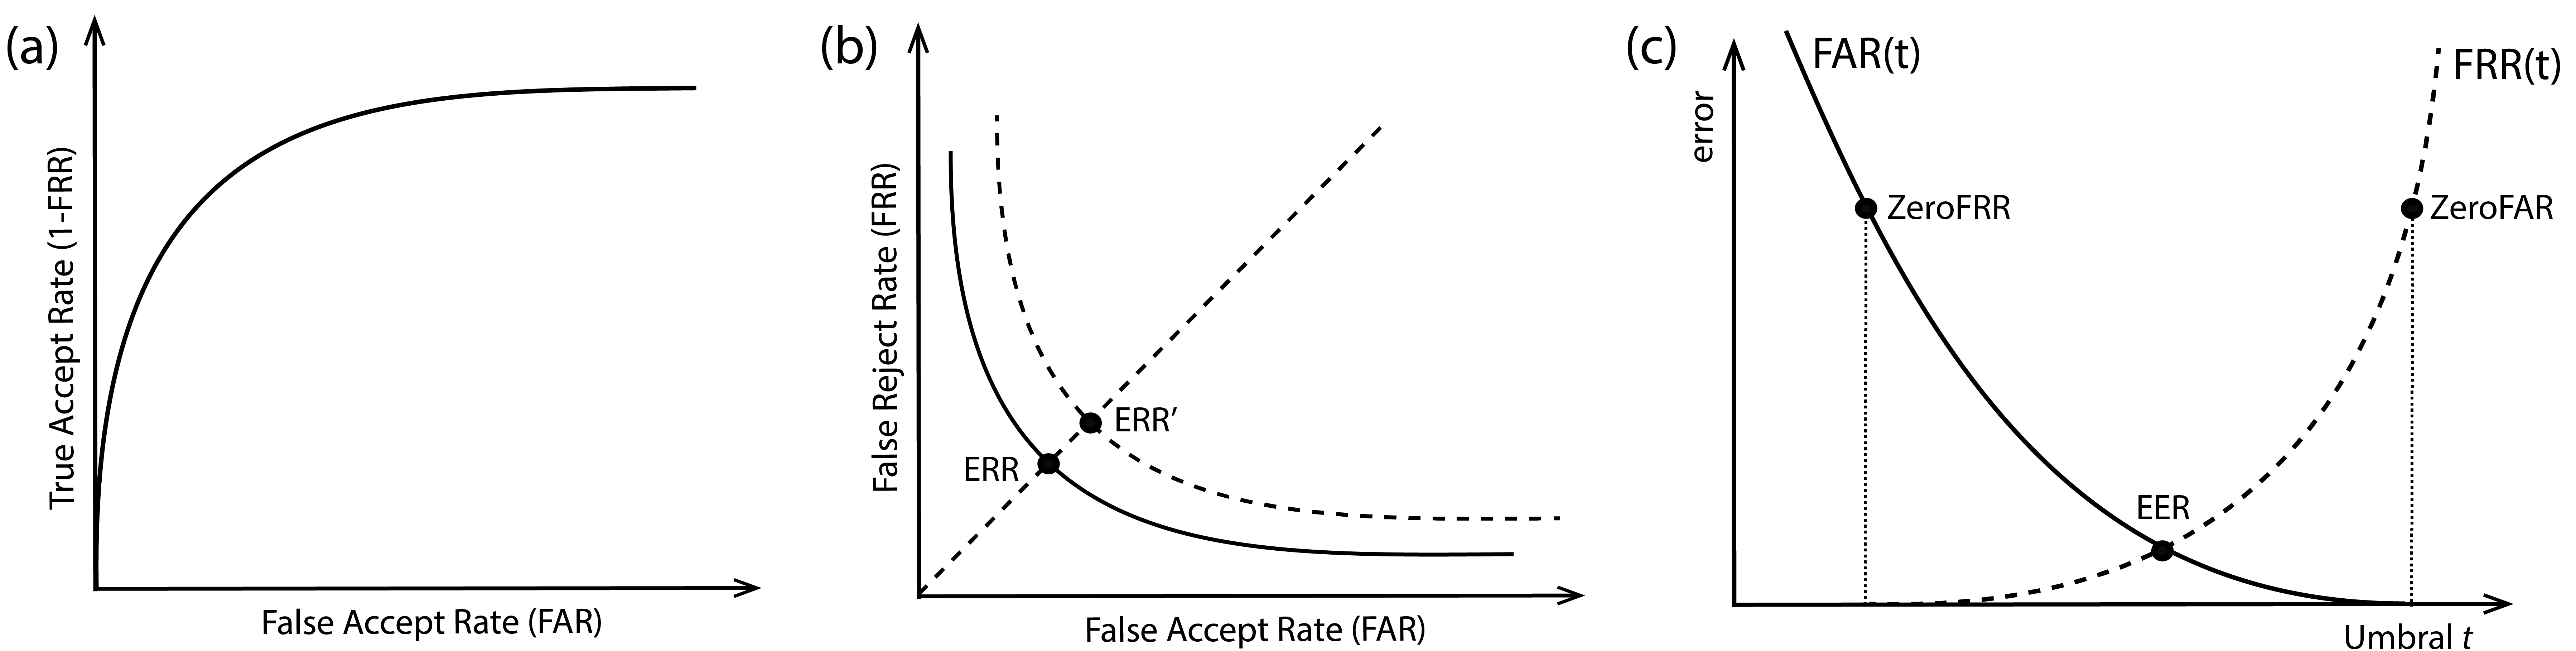
\includegraphics[width=0.9\textwidth]{ch-sistemasABC/images/ch-sistemasBiometricos/curves_ROC_DET_FARvsFRR-01.png}
    \caption{(a) Curva \GLS{ROC}. (b) Curva \GLS{DET}. (c) Curva \GLS{FAR}vs\GLS{FRR}.}
    \label{fig:tiposCurvas}
\end{figure}

Si el umbral se hace mas pequeño el sistema será más tolerante, aumentará el \GLS{FAR}(t), mientras que si el umbral es mayor, aumentará el \GLS{FRR}(t), se hará restrictivo.

Para visualizar el rendimiento de los sistemas biométricos se pueden dibujar dos tipos de curvas: \textit{Receiver Operating Characteristic} (\textbf{\GLS{ROC} curve}) y \textit{Detection Error Tradeoff} (\textbf{\GLS{DET} curve}). La curva \GLS{ROC} presenta e \GLS{FAR}(t) contra \textit{True Accept Rate} ($1$ - \GLS{FRR}(t)) para los distintos umbrales \textit{t} ver curva (a) en figura \ref{fig:tiposCurvas}. Mientras que la curva \GLS{DET} presenta el \GLS{FAR}(t) y el \GLS{FRR}(t) también para los distintos umbrales ver curva (b) en \ref{fig:tiposCurvas}. 

En ambas curvas cada punto de la curva se corresponde con un valor de umbral t.

Además de analizar visualmente las curvas para analizar el sistema, existen una serie de valores descriptivos del rendimiento del sistema, como el \textit{Equal Error Rate} \textbf{\GLS{EER}} o el \textbf{\textit{\Gls{ZeroFAR}}} o \textbf{\textit{\Gls{ZeroFRR}}} ver curva (c) en figura \ref{fig:tiposCurvas}.


%%%%%%%%%%%%%%%%%%%%%%%%%%%%%%%%%%%% BIOMETRIA:SEGURIDAD DE SISTEMAS BIOMÉTRICOS %%%%%%%%%%%%%%%%%%%%%%
\section{Ataques en sistemas biométricos}\label{sec:AtaquesSistemasbiometricos}

La introducción de datos biométricos en la seguridad requiere de nuevas medidas de protección, ya que si la información biométrica personal es robada, no es posible reemplazarla o sustituirla. De ahí que muchas investigaciones se centren en el estudio de medidas de protección y en la encriptación de este tipo de datos \cite{barni2010privacy} \cite{sasse2013usable}. 

Es necesario proteger la información tanto en su almacenaje como en las comunicaciones del sistema.

Otro de los aspecto de seguridad a tener en cuenta es la suplantación de identidad conocidos como \textit{\gls{spoofing}} o ataques de presentación, \cite{marcel2014handbook} \cite{marcel2019handbook}, \cite{ISO/PADFramework}.

Todos los subsistemas de un sistema biométrico son susceptibles de ser atacados. La imagen \ref{fig:esquemaSistemaBiometricoAtaques} muestra los puntos de un sistema biométrico donde se puede producir un ataque.

Es inevitable que surjan nuevos tipos de ataques a medida que aparecen nuevos materiales para la fabricación de artefactos y las instrucciones para fabricarlos se difundan más fácilmente.

\begin{figure}[t]
    \centering
    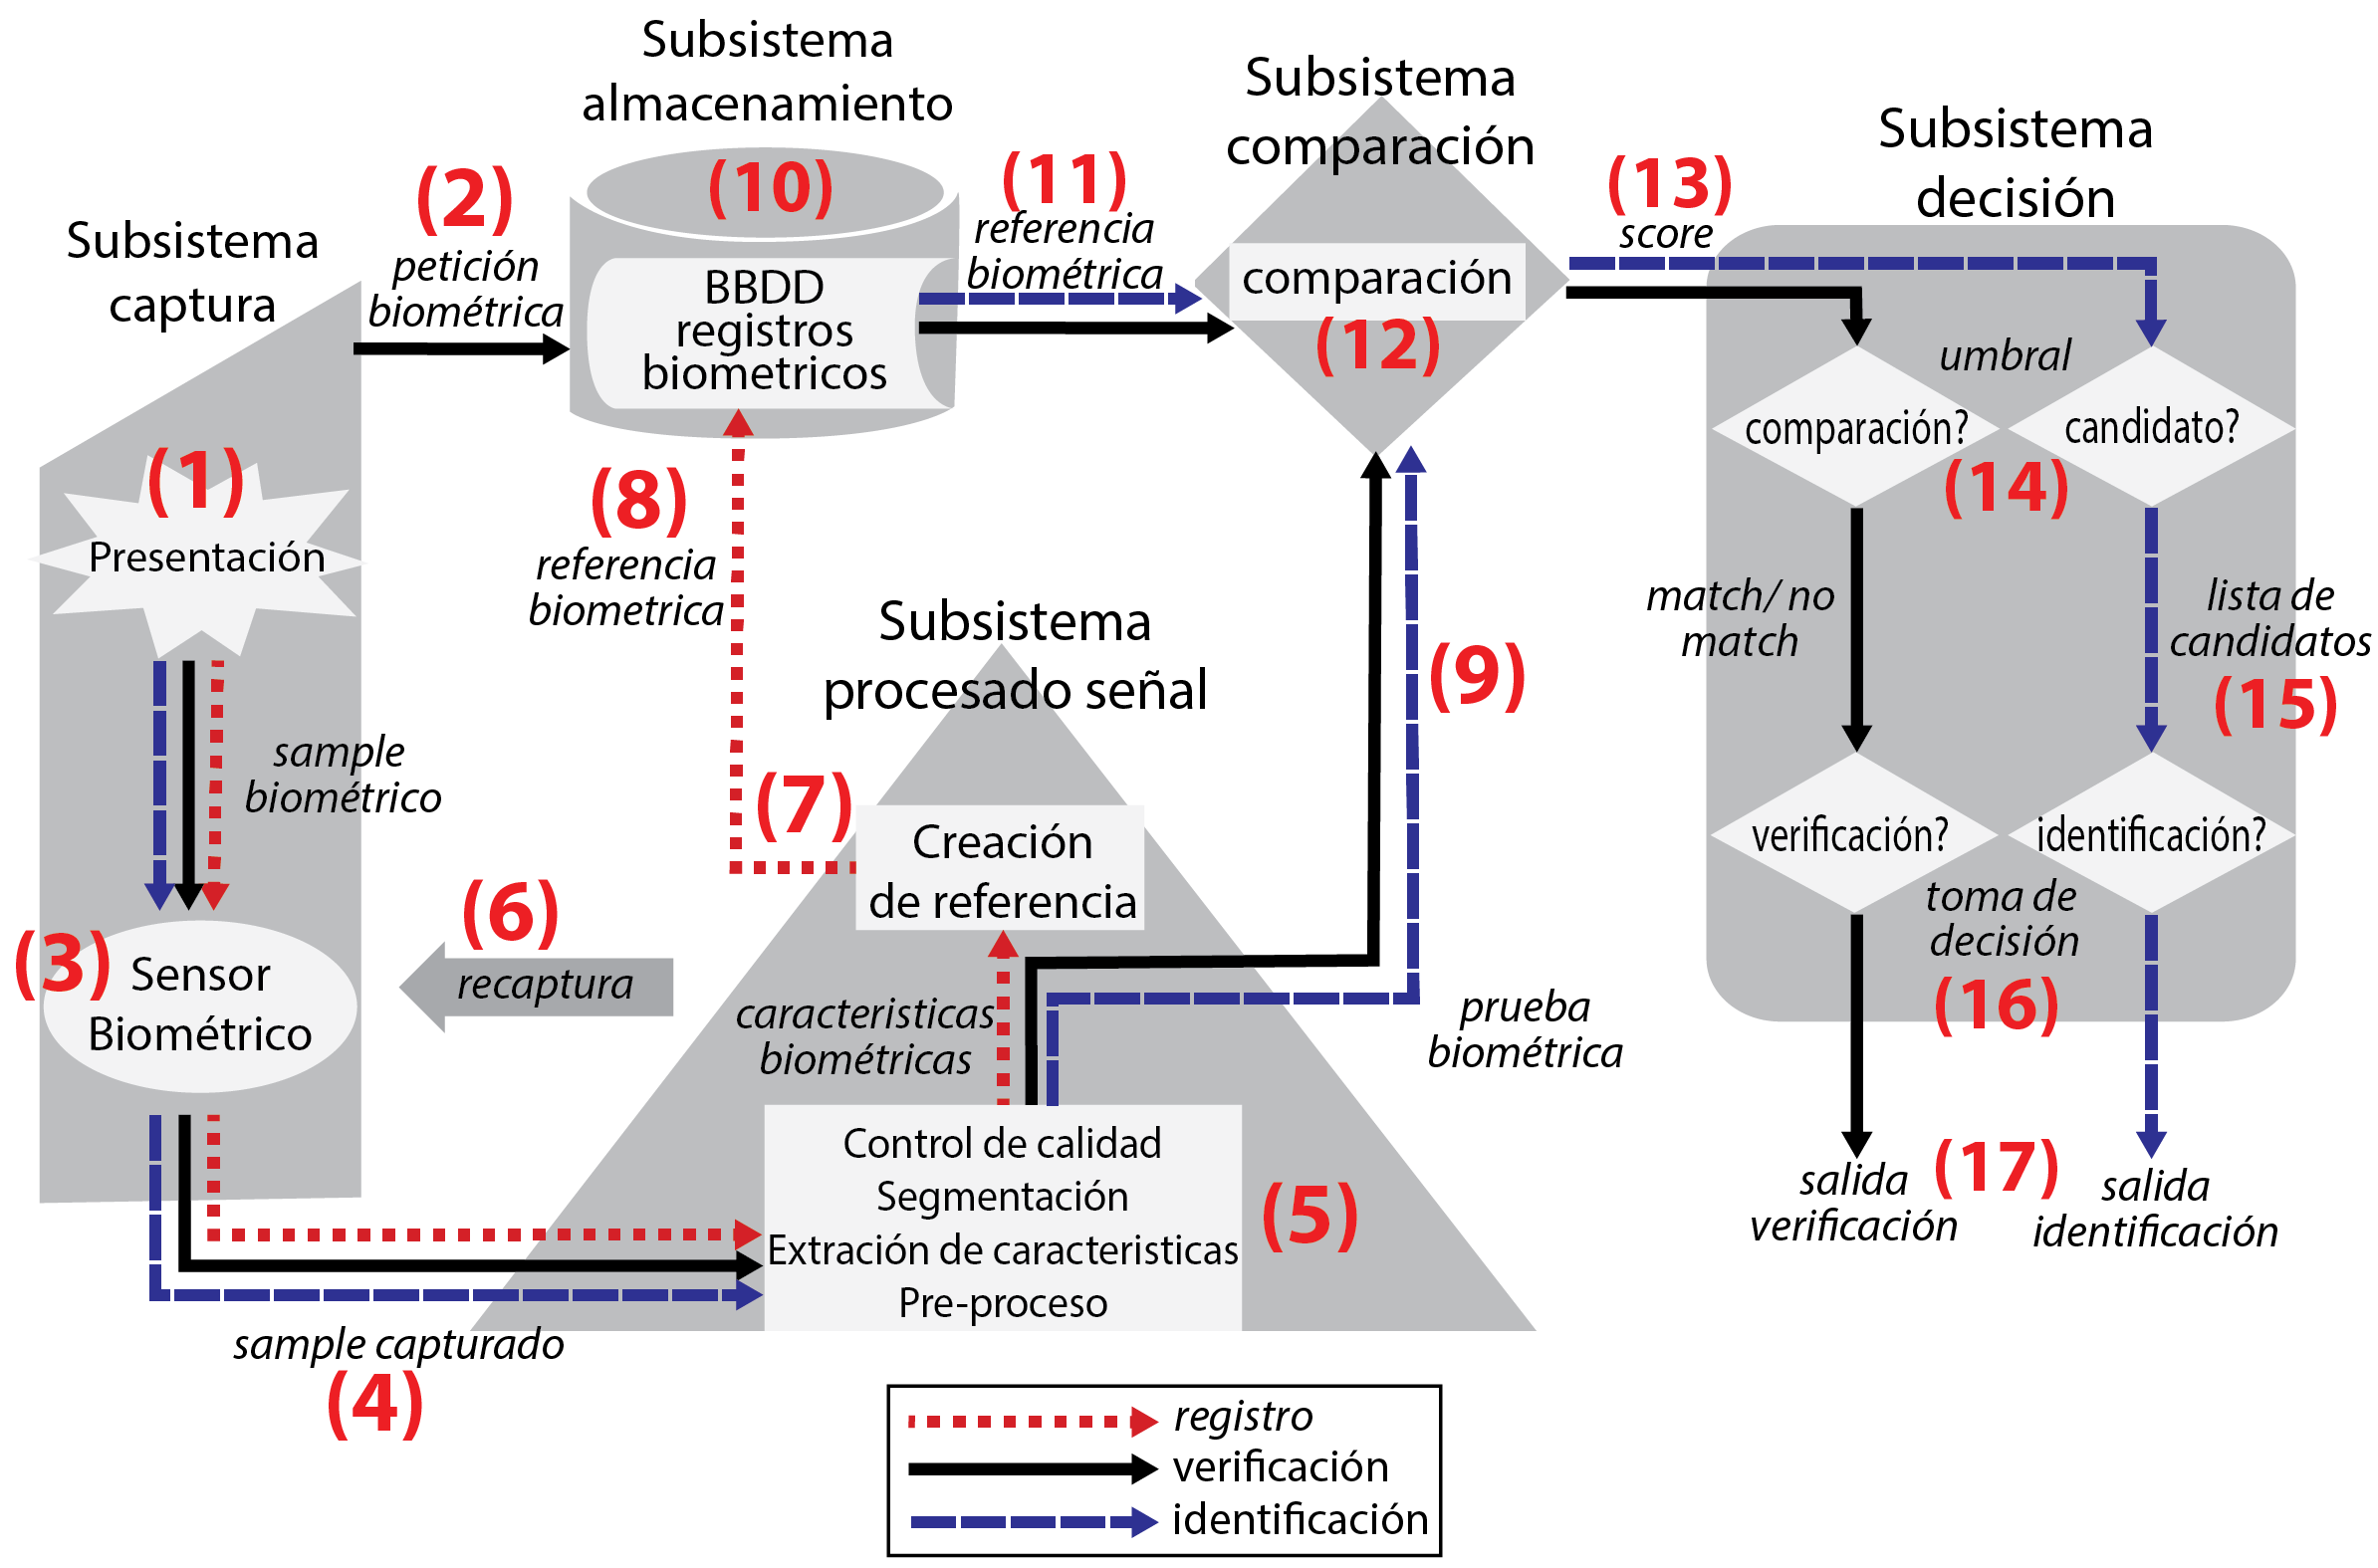
\includegraphics[width=0.8\textwidth]{ch-sistemasABC/images/ch-sistemasBiometricos/esquemaSistemaBiometricosAtaques.png}
    \caption{Ataques en un sistema biométrico \cite{ISO/Biometric}}
    \label{fig:esquemaSistemaBiometricoAtaques}
\end{figure}

\begin{itemize}
    \item 
    \textbf{(1) Ataque en la presentación}:
    Los ataques en este punto del sistema consisten en usar algún \textbf{artefacto} para \textbf{suplantar} el rasgo biométrico real, o en \textbf{alterar} u \textbf{ocultar} el rasgo biométrico propio. Dependiendo de la sofisticación del ataque, éste puede ser más o menos detectable.
    \item 
    \textbf{(2) Ataque en la identificación}:
    Este ataque consiste en el uso de documentación falsa, manipulada o robada. Una forma de llevar a cabo ataques de este tipo consiste en registrar los rasgos biométricos del atacante con la identidad a suplantar. Dependiendo del país, existe un mayor o menor control, a la hora de registrar una identidad. (En el capítulo \ref{ch:morphing} se analizan el ataque de morphing que es uno de estos tipos de ataques). 
    \item 
    \textbf{(3) Ataque en la sensor}:
    Este ataque consiste en manipular o reemplazar el sensor de captura de forma que se eviten ciertos controles de seguridad que el sensor original debería estar haciendo. (Por ejemplo, cambiar un lector de huellas con detección de huellas sintéticas por un sensor sin detección).
    
    Manipular el sensor de captura también puede usarse para el robo de rasgos biométricos, para un posterior ataque.
    
    Este ataque es difícil de llevar a cabo en sistemas de alta seguridad, donde los sensores están muy integrados con el resto del sistema, como los \GLS{ABC}. 
    \item 
    \textbf{(4) Ataque en la transmisión del rasgo}:
    El ataque consiste en interceptar la comunicación entre el sensor y el sistema de identificación. Los sistemas móviles son más sensibles a este tipo de ataques que los sistemas compactos, en los que se requeriría un mayor conocimiento interno del sistema.
    
    Interferir la lectura del chip en un \textit{\gls{eMRTD}} también se puede considerar un ataque de transmisión del rasgo. 
    \item 
    \textbf{(5) Ataque en la extracción de características o en el sistema de calidad}:
    Si no hay un estricto control de calidad del rasgo capturado es posible presentar un rasgo con poca calidad, por ejemplo una huella dactilar sucia o borrosa, y conseguir engañar al sistema.
    \item 
    \textbf{(6) Ataque en la recaptura}:
    Si no se limita el número de recapturas, el atacante puede ir modificando la presentación, hasta conseguir una aceptación por parte del sistema. 
    \item 
    \textbf{(7) Ataque en la creación de la plantilla de referencia}:
    Si se consigue acceder al módulo que construye las plantillas de referencia se puede modificar una de las plantillas de referencia para que valide con un determinado individuo. Este ataque requiere altos conocimientos de la implementación interna del sistema. 
    \item 
    \textbf{(8) Ataque en la transmisión de la plantilla de referencia}:
    De forma similar al ataque anterior se puede conseguir insertar en la base de datos de plantillas de referencia una plantilla que valide a un posterior atacante.
    \item 
    \textbf{(9) Ataque en la transmisión de las características}:
    Consiste en alterar las características extraídas del rasgo capturado, de forma que validen contra la plantilla de alguno de los usuarios registrados.
    \item 
    \textbf{(10) Ataque en el almacenamiento}:
    Insertar o modificar un registro de la base de datos.
    \item 
    \textbf{(11) Ataque en la transmisión de la plantilla de referencia al subsistema de almacenamiento}:
    Modificar la plantilla de referencia que va a usarse para realizar la comparación.
    \item 
    \textbf{(12) Ataque en el proceso de comparación}:
    Alterar el algoritmo de comparación para conseguir que devuelva un \textit{score} de semejanza alto entre una plantilla registrada y las características biométricas del atacante. 
    \item 
    \textbf{(13) Ataque en la transmisión del \textbf{score}}:
    Si se interceptan las comunicaciones entre el subsistema de comparación y el subsistema de decisión se puede alterar el \textit{score} de semejanza obtenido y engañar al sistema de decisión.
    \item 
    \textbf{(14) Ataque en proceso del umbral}:
    Alterar el umbral usado para tomar una decisión, de forma que se cual sea el \textit{score} de semejanza obtenido por el rasgo presentado, el resultado sea una aceptación.
    \item 
    \textbf{(15) Ataque en la lista de candidatos}:
    Cuando el sistema está realizando una identificación, se puede atacar la lista de cándidos, añadiendo uno nuevo o eliminando alguno, para que el atacante sea o no identificado por el sistema., dependiendo si el ataque es una ocultación o una suplantación. 
    \item 
    \textbf{(16) Ataque en la toma de decisiones}:
    Accediendo al sistema de decisión el atacante puede alterar el resultado final. 
    \item 
    \textbf{(17) Ataque en la transmisión de la decisión}:
    Accediendo la transmisión de salida del subsistema de decisión, se puede alterar el resultado final del sistema. 
\end{itemize}    

\textbf{Ataque en la administración del sistema}: Además de los ataques a los subsistemas físicos del sistema biométrico, también es posible que el ataque afecte al control interno o a la administración del sistema en sí. Accediendo a los propios sistemas de control o bien mediante un colaborador dentro del equipo administrativo. 
    
\textbf{Ataque al sistema de detección de ataques de presentación}: Algunos sistemas biométricos disponen de subsistemas de detección de ataques de presentación. Y estos subsistemas también son susceptibles de ser atacados, de forma que no se detecten ataques de presentación y dejen al sistema expuesto a ellos.
    

%%%%%%%%%%%%%%%%%%%%%%%%%%%%%%%%%%%% BIOMETRIA:FALLOS EN LOS SISTEMAS BIOMETRICOS %%%%%%%%%%%%%%%%%%%%%%
\section{Fallos en los sistemas biométricos.}\label{sec:fallosBiometricos}

% \color{cyan}Los errores habituales en cualquier sistema biométrico son la falsa aceptación y el falso rechazo.\color{black} 


La reducción de la interacción humana en los sistemas biométricos hace que se incrementen los riesgos de seguridad y que requieran unas medidas de control especificas.

Todos los errores deberían quedar registrados en el sistema para que con futuros controles de calidad y de satisfacción puedan ser detectados, analizados y subsanados.

En los sistemas \GLS{ABC} se pueden considerar errores de tres tipos: \textbf{Errores técnicos}, producidos por el mal funcionamiento del sistema y \textbf{errores operacionales} causados algún comportamiento indebido del viajero. 

\paragraph{Errores técnicos}:

Son los fallos eléctricos, mecánicos o de conexión.

También son los errores causados por deterioro o suciedad en los sensores que dificulta o impide la adquisición correcta.

Errores en las operaciones o comunicaciones internas del sistema (Fallos en el protocolo de comunicaciones o incompatibilidad de formatos de imagen) 

Son fáciles de localizar si el sistema está bien trazado, combine que las trazas del sistema estén organizadas por niveles, para identificar más rápidamente la causa de estos errores.  

\paragraph{Errores operacionales}:

Los errores operacionales son los errores producidos por le mal uso del sistema. Este mal uso puede estar provocado por el propio usuario o puede producirse de manera involuntaria por fallos en el diseño del sistema. Normalmente los fallos en diseño del sistema degeneran en fallos del usuario. 

Son más difícilmente detectables y reproducibles que los errores técnicos ya que estos errores suelen terminar en un falso rechazo sin causa aparente. 
\textbf{Errores operacionales provocados por el viajero}:
\begin{itemize}
    \item 
    Colocar el dedo incorrecto sobre el sensor.
    \item
    No colocarse en la pose correcta para la captura \gls{facial}.
    \item
    Llevar algún complemento no permitido que oculte el rasgo biométrico: gafas de sol, bufandas, gorra, etc. 
    \item
    Retirar el pasaporte o moverlo en el escáner antes de que que haya podido ser leído. 
    \item
    Mover el dedo o la cara mientras se está produciendo la adquisición. Esto produce capturas de baja calidad.
\end{itemize}

\textbf{Errores operacionales por las características del sistema}:
\begin{itemize}
    \item 
    Lector de huellas erróneamente colocados. Por ejemplo, solicitar la mano derecha cuando el lector está a la derecha.
    \item
    No colocar un espejo o algún sistema que sirva al usuario para controlar su pose.  
    \item
    Interfaz mal diseñado o colocado de forma que dificulte la interacción del usuario.
\end{itemize}

Este tipo de errores se pueden minimizar si se toman las medidas de usabilidad adecuadas, descritas en el punto 
%\ref{sec:ErgonomiaBiometricosABC}. 
O si los sistemas de adquisición se hacen más robustos con métodos de medición de la calidad de la adquisición o tomando varias capturas de un mismo rasgo. 
% \color{cyan} quizás aquí pega la imagen con el sistemas de medición calidad de la adquisición\color{black}.


%%%%%%%%%%%%%%%%%%%%%%%%%%%%%%%%%%%% ABC_BIOMETRICO:BIOMETRIA FACIAL EN ABC %%%%%%%%%%%%%%%%%%%%%%
\section{Biometría facial en los ABC}\label{sec:BiometriaFacialABC}

La cara es la \gls{biometria} mas natural ya que es la forma en la que tenemos los seres humanos de identificarnos.

Usar la \gls{biometria} \gls{facial} como rasgo para la identificación biométrica tiene una serie de ventajas:
\begin{itemize}
    \item 
    Tiene una alta aceptación, para la mayoría de las culturas.
    \item
    Su \gls{captura} resulta muy poco intrusiva, en comparación con otras \glspl{biometria}.
    \item
    Los agentes de seguridad están familiarizados con el concepto de verificación \gls{facial}.
\end{itemize}

Por estas razones ICAO, incluye en los estándares para la primera generación de \textit{\gls{e-passport}} una imagen \gls{facial}. Tanto ISO/EIC en ISO/EIC 19794-5 como ICAO \cite{doc20069303} establecen una serie de requisitos que deben cumplir estas imágenes con el fin de facilitar la verificación \gls{facial} \cite{jafri2009survey} \cite{del2015face}.

El rendimiento de los reconocedores faciales se ve alterado por las condiciones de: iluminación, pose, oclusión expresión, resolución y otros factores que reducen su fiabilidad.

Algunos estudios tratan de hacer frente a estos problemas. Por ejemplo \cite{abiantun2014sparse} propone modelos elásticos 3D para hacer frente al problema de la pose.

\color{red} quizás una tabla con las problemáticas y con los papers que se enfrentan a dicha problemática y con que algoritmo \color{black}

\color{red} AÑADIR DE ALGUIEN POSANDO DELANTE DE UN ABC \color{black}

% Para llevar un control de la calidad y del rendimiento del sistema biométrico, es necesario guardar \textbf{trazas de cada una de las operaciones} que realiza. Por cada una de las operaciones se debe guardarse:

% \begin{itemize}
%     \item
%     El \textbf{\textit{score} de verificación} resultante y el \textbf{\textit{score} de calidad} de la captura del rasgo.
%     \item
%     El \textbf{umbral de aceptación} que se está usando tanto para el \textit{score} de verificación como para el \textbf{score} de calidad.
%     \item
%     Los \textbf{Errores} producidos.
%     El \textbf{tiempo completo} del proceso desde que se realiza la captura hasta que se obtiene un resultado.
%     \item
%     El \textit{tiempo de adquisición} que es el tiempo transcurrido desde que comienza el proceso de adquisición hasta que se consigue capturar el rasgo y permite evaluar los retrasos que se producen por el comportamiento del viajero.
% \end{itemize}

% Es siempre recomendable usar métodos de \GLS{PAD} y de \gls{liveness detection}, (Ver capitulo \ref{ch:PAD}).

% Los estándares de \GLS{ISO}/\GLS{IEC} $19794$ \cite{ISO/Format} para formatos de imagen en sistemas biométricos recomiendan el uso de imágenes de tipo \GLS{PNG} o \GLS{JPG2000}, sin compresión para evitar la perdida de información. 
% Dentro de las trazas de los sistemas \GLS{ABC} se debería añadir un traza especificas del sistema biométrico, que incluya información como:
% \begin{itemize}
%     \item
%     \textit{Score} de oclusión.
%     \item
%     \textit{Score} de pose, especialmente en las \gls{biometria} \gls{facial} y en la \gls{biometria} del \gls{iris}.
%     \item
%     \textit{Score} de ruido.
%     \item
%     \textit{Score} de opacidad en las gafas, especialmente en la \gls{biometria} del \gls{iris}.
% \end{itemize}

\color{red}
\GLS{ICAO} en doc $9303$ \cite{doc20069303} define la cara como \textbf{primer rasgo biométrico} para los documentos \gls{eMRTD}.


Los componentes a tener en cuenta en la \gls{biometria} \gls{facial}:

\begin{itemize}
    \item
    \textbf{Cámaras de adquisición:} Cámaras que puedan adaptarse a las distintas alturas de los viajeros.
    \item
    Sistemas de \textbf{iluminación:} Luz uniforme y simétrica que no deslumbre al viajero y que compense las luces de ambiente.
    \item
    Módulo de \textbf{evaluación de la calidad}: Modulo que garantice la calidad de la imagen para que la verificación funcione correctamente, rechazando que no permitan extraer las características del rasgo. Debe comprobar que la captura cumple los estándares fijados por \GLS{ICAO}en doc $9303$ \cite{doc20069303} y \GLS{ISO}/GLS{IEC} $19794$-$5$:$2011$ \cite{ISO/Face}. APENDICE CON LA CARA?
    \item
    Modulo de verificación facial: Compara la imagen capturada con la imagen almacenada en el documento o con la imagen almacenada en la base de datos, dependiendo del tipo de sistema.
\end{itemize}

Los pasos de proceso de biometria facial son:

\begin{enumerate}
    \item 
    El viajero se acerca o entra al dispositivo dependiendo del tipo.
    \item
    Se selecciona la cámara en la que se detecta la cara del viajero. En el caso de que se trate de una cámara ajustable, ésta se desplazará hasta encontrar la cara del viajero.
    \item 
    Se indica al viajero la pose que debe tomar.
    \item
    El sistema de iluminación se ajusta para corregir los problemas generados por la luz de ambiente.
    \item
    Si el modulo de calidad de imagen del sistema no considera que la imagen pueda ser verificada, se puede solicitar al viajero una recaptura, solo un número determinado de veces para garantizar la seguridad del sistema (ver punto que habla de esto).
    \item
    Cuando la imagen tiene la calidad suficiente se compara la imagen de la cara capturada con la imagen almacenada en el pasaporte o con la almacenada en la base de datos, depende el tipo de sistema. 
\end{enumerate}

\color{black}


%%%%%%%%%%%%%%%%%%%%%%%%%%%%%%%%%%%%  ABC_BIOMETRICO:ADQUISICÓN FACIAL ABC %%%%%%%%%%%%%%%%%%%%%%
\subsubsection{Adquisición en la biometría facial}\label{subsec:AdquisicionFacialABC}

Para el diseño de los sistemas \GLS{ABC}, es conveniente tener en cuenta otra serie de medidas cuando la biometría empleada es facial;

\begin{itemize}
    \item
    Hacer que la dirección del flujo de pasajeros y la \textbf{orientación del dispositivo} de captura no difieran en más de $45$º ya que esto ralentizaría el flujo de pasajeros.
    
    \item
    Evitar que el viajero tenga que realizar alguna acción que pueda distraerle durante la adquisición. Y colocar los elementos del \textit{interface} del sistema (botones, pantallas, leds, etc.) lo más cerca posible del dispositivo de captura, para que el viajero \textbf{no tenga necesidad de desviar la mirada}.
    
    \item
    La \textbf{profundidad de campo} de la cámara depende del tipo de dispositivo \GLS{ABC} (\gls{mantrap}, \gls{e-kiosk}, etc.), pero preferiblemente debe ajustarse al área donde normalmente se sitúa la cara, para de está forma, evitar problemas con el fondo de la imagen capturada. 
    
    \item
    Cuando la captura sea un vídeo se recomienda una velocidad de grabación de al menos de \textbf{$10$ \textit{frames per second} (fps)}.
    
    \item
    Conseguir que la imagen capturada cumpla las mismas \textbf{especificaciones que fija \GLS{ICAO} doc $9303$ \cite{doc20069303}} para las imágenes faciales de los \GLS{eMRTD}, facilitará una posterior verificación. Por ejemplo, la imagen de la cara capturada debe tener al manos $90$ píxeles entre los centros de los ojos.
    
    \item
    El sistema debe estar preparado para capturar el rostro de forma frontal de viajeros con una estatura entre $140$  y $200$ cm. Para ello se pueden usar varias estrategias para realizar la \textbf{adquisición frontal a distintas alturas}.
    \begin{itemize}
    \item 
    Cámaras móviles
    \item
    Cámaras basculantes.
    \item
    Espejos móviles.
    \item
    Lentes con gran amplitud de campo.
    \item
    Varias cámaras a distintas alturas.
    \end{itemize}

    \item
    Tratar que la zona del rostro tenga una \textbf{buena iluminación}, evitando los efectos del contraluz o reflejos en los cistales de las gafas o en la piel del viajero.
    
    \item
    En la medida de lo posible se debe \textbf{minimizar el tiempo} de la captura. Por ejemplo, Hacer \textbf{\textit{tracking}} de la cara desde que el viajero se sitúa frente al dispositivo, puede hacer que la captura sea mas rápida y precisa. 
    
    \item
    Es recomendable usar un \textbf{espejo} para que el viajero pude comprobar su pose. Si en vez de un espejo, se presenta un vídeo con lo que está capturando la cámara (\textbf{espejo digital}), se pueden incluir indicaciones al viajero para que corrija su pose o avisarle cuando la cara está correctamente colocada. \color{cyan} referenciar aquí lo de el sistema de mediccion de la calidad de la captura cuando lo meta en algún sitio, debería estar en sistemas biométricos \color{black} 
    
    \item 
    Si se emplean \textbf{cámaras de alta resolución} se evita el uso del zoom o de lentes que pueden producir efectos de desenfoque o imágenes ruidosas.  
    
    \item
    Intentar evitar la perdida de de información, que puede resultar contraproducente para los algoritmos de verificación, por culpa de la \textbf{compresión de la imágenes}\footnote{\GLS{ISO}/\GLS{IEC} $194794$-$5$ \cite{ISO/BioApi} propone una serie de recomendaciones para los formatos de imagen que deben usarse en los sistemas \GLS{ABC}.}.
\end{itemize}

\begin{figure}[t]
    \centering
    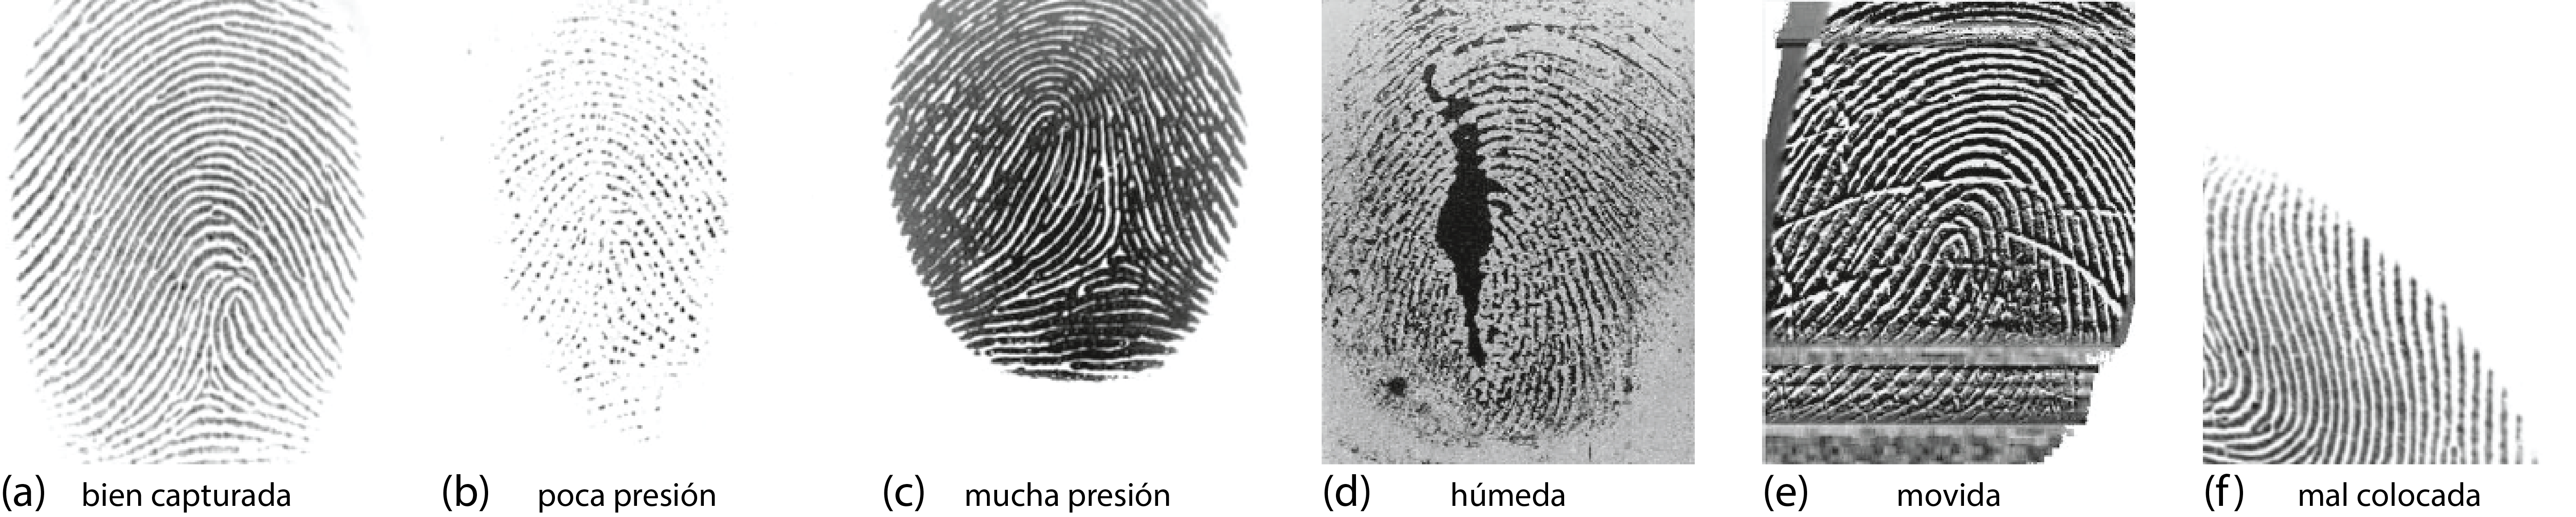
\includegraphics[width=1\linewidth]{ch-sistemasABC/images/ch-biometricosABC/adquisicionesDactilares.png}
    \caption{Tipos de adquisición de huellas dactilares \cite{ted2008biometric}.}
    \label{fig:AdquisicionDactilares}
\end{figure}



%%%%%%%%%%%%%%%%%%%%%%%%%%%%%%%%%%%%  ABC_BIOMETRICO:VERIFICACION FACIAL ABC %%%%%%%%%%%%%%%%%%%%%%
\subsubsection{Verificación en la biometría facial}\label{subsec:VerificacionFacialABC}

La verificación \gls{facial} debe realizarse siempre que sea posible con la imagen almacenada en el chip del \gls{eMRTD} y \textbf{no con la imagen de la zona \GLS{VIZ}} del documento, que al estar impresa, tiene menos calidad y además puede estar deteriorada.   

No debería tardar más de \textbf{30 segundos}, contando la adquisición  y el proceso de lectura de la información almacenada en el \gls{eMRTD}.

Es recomendable que el rendimiento del verificador sea al menos de un \textbf{\GLS{FAR}} del $0,1$\% y comprobar que para ese \GLS{FAR} el \textbf{\GLS{FRR}} no debe superar el $5$\%.  

Los sistemas de verificación facial están en continua evolución y mejora, por lo que es recomendable al menos, \textit{revisarlo una vez al año}, evaluando sus \GLS{FAR} y \GLS{FRR}.



%%%%%%%%%%%%%%%%%%%%%%%%%%%%%%%%%%%%  ABC_BIOMETRICO:BIOMETRIA DACTILAR EN ABC %%%%%%%%%%%%%%%%%%%%%%
\section{Biometría huella dactilar en los ABC}\label{subsec:BiometriaDactilarABC}

Las huellas dactilares son los patrones complejos que se forman en la yemas de los dedos durante la gestación. Son únicos en cada individuo y al no tener una implicación genética incluso los hermanos gemelos tienen huellas dactilares diferentes entre si. Son unos de los primeros rasgos biométricos usados para la identificación, primero en el campo de la criminología pero, actualmente, su usó esta completamente extendido, siendo uno de los rasgos más comunes en los sistemas biométricos.

Las huellas dactilares son otro de los rasgos más habituales en los sistemas \GLS{ABC} desde que \gls{ICAO} añadió las huellas dactilares como rasgo  opcional, además de la cara, para la segunda generación de \textit{\gls{e-passport}}.

También existe un estándar (\GLS{ISO}/\GLS{EIC} $19794$-$4$) que especifica los requisitos de calidad que deben tener las imágenes de huella dactilar almacenadas en el los \textit{\gls{e-passport}}. 

Aunque las tasas de reconocimiento y verificación alcanzadas por la \gls{biometria} dactilar son altas, factores como la suciedad en el sensor o en las manos, hacen que su rendimiento se vea muy mermado.

Gran parte de los problemas de la biométrica \gls{facial} vienen del proceso de adquisición \cite{labati2015automatic}.


Es una rasgo susceptible de suplantación mediante la construcción de huellas falsas o directamente mediante dedos reales amputados o de cadáveres

Huellas sintéticas construidas con la colaboración del viajero a suplantar o sin colaboración, mediante huellas latentes \cite{galbally2011evaluation} \cite{espinoza2011vulnerabilities}.

\color{red}En los años $70$ Shearon Nonil Indetimat creó el primer centro de acceso mediante huella dactilar\color{black}

El primer uso de que se le dio a la identificación con huellas dactilares en el terreno judicial para identificar criminales.

En $1979$ US Federal Bureau of Investigation empezó a usar el primer sistema automático de verificación de huellas y en $1983$ creó la primera aplicación para ser usada a tiempo real. \textit{Automated Fingerprint Identification System \GLS{AFIS}}.

Es una biométrica con sensores baratos.

La mayoría de los sistemas \GLS{ABC} usan sensores ópticos con imágenes de alta resolución.

Determinadas condiciones dificultan o incluso imposibilitan la lectura de las huellas dactilares 

\begin{itemize}
    \item 
    Por \textbf{condiciones médicas}: 

    Los \textbf{cambios de peso}

    Determinados \textbf{medicamentos} contra el cáncer borran las huellas dactilares. (http://news.bbc.co.uk/z/hi/healdrth/8064332.stm)

    \textbf{Artritis}, \textbf{Parkinson} u otras enfermedades dificultan colocar as manos en sensor.
    
    \item
    Por \textbf{ocupación}:
    
    Algunas profesiones usan \textbf{sustancias abrasivas} que borran las huellas dactilares.
    
    \item
    Por \textbf{condiciones de viaje}:
    
    La \textbf{presión} de cargar el equipaje dificulta la lectura.
    
    La \textbf{suciedad}.
    
    \item
    Por \textbf{etnia}:
    
    Algunas etnias, como los orientales, tienen los \textbf{rasgos dactilares menos señalados}, lo que dificulta su lectura.
    
\end{itemize}



\color{red}
No todos los pasaportes tienen  información sobre la huella dactilar del viajero. \GLS{ICAO} en doc $9303$ \cite{doc20069303} establece las huellas dactilares como rasgo biométrico opcional.

Es un rasgo biométrico muy preciso y socialmente aceptado.

El $61$\% de los sistemas \GLS{ABC} en \GLS{EU} usan las huellas dactilares para la verificación de la identidad del viajero.

Los principales componentes del sistema de \gls{biometria} \gls{dactilar}:

\begin{itemize}
    \item 
    Escáner de huellas dactilares: Los sistemas \GLS{ABC} pueden usar una única huella o cuatro. Normalmente son sensores ópticos, pero se pueden encontrar otro tipo de sensores (ver \ref{sec:AdquisicionDactilarABC}).  
    \item
    Modulo de evaluación de calidad de la imagen dactilar: Debe garantizar la calidad de la imagen de la huella para ser verificable. Debe comprobar que se cumplan los estándares \GLS{ISO}/\GLS{IEC} $19794$-$4$ \cite{ISO/Finger} y NIST Finger Print Image Quality (\GLS{NFIQ}).
    \item
    Módulo de verificación facial: Se compara la imagen de la huella capturada por el sistema con la almacenada en el documento o en la base de datos. Uno de los métodos de verificación más usados es la comparación de minucias \cite{gamassi2005fingerprint}\cite{gamassi2005robust}\cite{maltoni2009handbook}. 
\end{itemize}

Los pasos del proceso de la \gls{biometria} \gls{dactilar}:

\begin{enumerate}
    \item
    Si el dispositivo lo permite, se ajusta automáticamente la altura del sensor y del ángulo.
    
    \item
    Debe indicarse al usuario que dedo debe colocar en el lector. A veces el dedo a colocar se selecciona de forma aleatoria de forma que se pueda verificar el \gls{liveness} del viajero.
    
    \item
    Se evalúa la calidad de la la imagen capturada, si no tiene la calidad suficiente para extraer las características a verificar se solicita una recaptura del rasgo.
    
    \item
    Si el sistema requiere más de una huela, se solicitan el resto delas huellas.
    
    \item
    Se compara la huella o huellas con las almacenadas en los documentos o en el la base datos dependiendo del tipo de sistema. 
    
\end{enumerate}

Los principales retos en la \gls{biometria} \gls{dactilar} son:

\begin{itemize}
    \item 
    Es necesario desarrollar sistemas para evaluar la calidad de la huella.
    
    \item
    Resulta necesario estandarizar la encriptación de los datos biométricos entre países para facilitar el acceso conservando la seguridad. 
    
    \item
    Reducir los tiempo de adquisición con sensores más rápidos y con algoritmos de evaluación de calidad y de verificación más optimizados.
    
    \item
    Mejorar los sistemas de \GLS{PAD} \cite{marasco2015survey}.
\end{itemize}

\color{black}


%%%%%%%%%%%%%%%%%%%%%%%%%%%%%%%%%%%%  ABC_BIOMETRICO:ADQUISICION DACTILAR EN ABC %%%%%%%%%%%%%%%%%%%%%%
\subsubsection{Adquisición en la biometría dactilar}\label{sec:AdquisicionDactilarABC}

Existen distintos tres tipos de \textbf{tecnologías} especializadas en la \textbf{captura} de huellas dactilares: Sensores ópticos, sensores de estado solido, sensores de ultrasonido. 

\begin{itemize}
    \item 
    \textbf{Lectores ópticos}:
    
    Este tipo de lectores usan \textbf{sensores ópticos}, similares a los de las caparas digitales, \textbf{\GLS{CCD}} o \textbf{\GLS{CMOS}}.
    
    \textbf{FTIR-Reflexión interna} (\textit{Frustrated Total Internal Reflexion}):
    
    Mediante un \textbf{sensor óptico} se lee la luz que atraviesa un \textbf{prisma} (ver (a) en Figura \ref{fig:SensoresDactilares}). Los valles permiten el paso de la luz por lo que en la imagen aparecerán en blanco, mientras que las crestas no permiten el paso de la luz, por lo que en la imagen aparecen en negro.
    
    Este tipo de sensores no pueden ser engañados mediante una fotografía ya que ésta no permite el paso de la luz. 
    
    \textbf{FTIR-Lámina de prismas}:
    
    Es una versión del tipo de sensor anterior en la que se reemplaza el prisma por una \textbf{lámina de pequeños prismas} con las que se consigue una \textbf{mayor resolución} en la imagen capturada (ver (b) en Figura \ref{fig:SensoresDactilares}).
      
    \textbf{FTIR-Fibra óptica} (\textit{Frustrated Total Internal Reflexion}):
    
    Otra versión del sensor \textbf{\GLS{FTIR}} en el que la \textbf{fuente de luz} es reemplazada por \textbf{fibra óptica}, lo que hace el sensor más \textbf{compacto} y reduce considerablemente su tamaño (ver (c) en Figura \ref{fig:SensoresDactilares}). 
    
    \textbf{Electro-opticos}:
    
    Formado por un \textbf{polímero sensible} que emite luz dependiendo de la \textbf{presión} que se le aplica y una \textbf{lamina fotosensible} (lamina de fotodiodos) que convierte la luz emitida en imagen  (ver (d) en Figura \ref{fig:SensoresDactilares}). Al estar las crestas en relieve emiten más luz que los valles, esto hace que imagen capturada será inversa a la obtenida por los sensores \textbf{\GLS{FTIR}}.  
    
    Este tipo de sensores tampoco pueden ser engañados por una fotografía ya que detecta el volumen de la huella.   
    
    \textbf{De lectura directa}:
    
    Captura la huella con una \textbf{cámara de alta resolución}, por lo que no requiere un contacto directo entre la huella y el sensor, lo que hace que sea un proceso más higiénico. Pero, al no tener contacto, resulta difícil conseguir una imagen nítida por lo que se puede colocar un soporte para ser conseguir imágenes más uniformes. 
    
    \textbf{Imágenes multiespectrales}:
    
    Usan una \textbf{iluminación con distintas frecuencias de onda} para leer huellas en condiciones no óptimas de iluminación y capturar determinadas características de la piel que permiten detectar huellas sintéticas.
    
    \item
    \textbf{Sensores de estado solido}:
    
    La huella se coloca sobre una \textbf{matriz de sensores} de silicio que captura una imagen en la que \textbf{cada sensor es un píxel} (ver (e) en Figura \ref{fig:SensoresDactilares}). Dependiendo del tipo de sensores existen diferentes lectores.
    
    \textbf{Capacitivos}:
    
    Basado en \textbf{sensores capacitivos} que crean cargas eléctricas entre la superficie del dedo y el sensor. Dependiendo de la proximidad al sensor la carga generada sera menor o menor, lo que genera un patrón con las crestas y los valles. 
    
    Este tipo de sensores son capaces de detectar suplantaciones con una fotografías o con huellas sintéticas que no tienen capacidad de transmisión eléctrica.
    
    Para que este tipo de sensores funcionen correctamente requieren una lamina protectora muy fina, lo que los hace \textbf{muy sensibles}. Se deterioran fácilmente con el sudor y requieren una limpieza continua para evitar la \textbf{corrosión química}. 
    
    \textbf{Térmicos}:
    
    En este tipo de lectores usa \textbf{sensores térmicos} que generan un \textbf{diferencial térmico} entre la huella y el lector. La diferencia de temperatura entre valles y crestas se convierte en una imagen.  
    Son más robustos que los lectores capacitivos ya que pueden protegerse mejor, pero se ven \textbf{afectados por las condiciones climáticas externas}.
    
    \textbf{Radio-frecuencia}:
    
    Emite una señal de \textbf{radio-frecuencia} y lee la respuesta de la señal al rebotar en la \textbf{epidermis}. Con la intensidad de la respuesta de la señal genera la imagen de la huella. Este tipo de sensores requiere un \textbf{contacto directo} con la superficie del dedo.  
    
    \textbf{Piezo-eléctricos}:
    
    Usa \textbf{sensores sensibles a la presión}, produciendo una señal eléctrica dependiendo de la presión ejercida. Con esas señales eléctricas producidas se genera la imagen de la huella.
    
    \item
    \textbf{Sensores de ultrasonido}:
    
    Lee los rasgos dactilares mediante reflexión acústica.
    
    El lector envía una serie de \textbf{señales con pulsos acústicos} y la lee el \textbf{eco} producido por el dedo  (ver (f) en Figura \ref{fig:SensoresDactilares}). Con este eco se calcula la \textbf{profundidad de las crestas y de los valles} componiendo la imagen de la huella. Estos sensores son \textbf{caros} y algo \textbf{lentos} ya que tardan unos pocos segundos en realizar la lectura.
    
\end{itemize}

\begin{figure}[t]
    \centering
    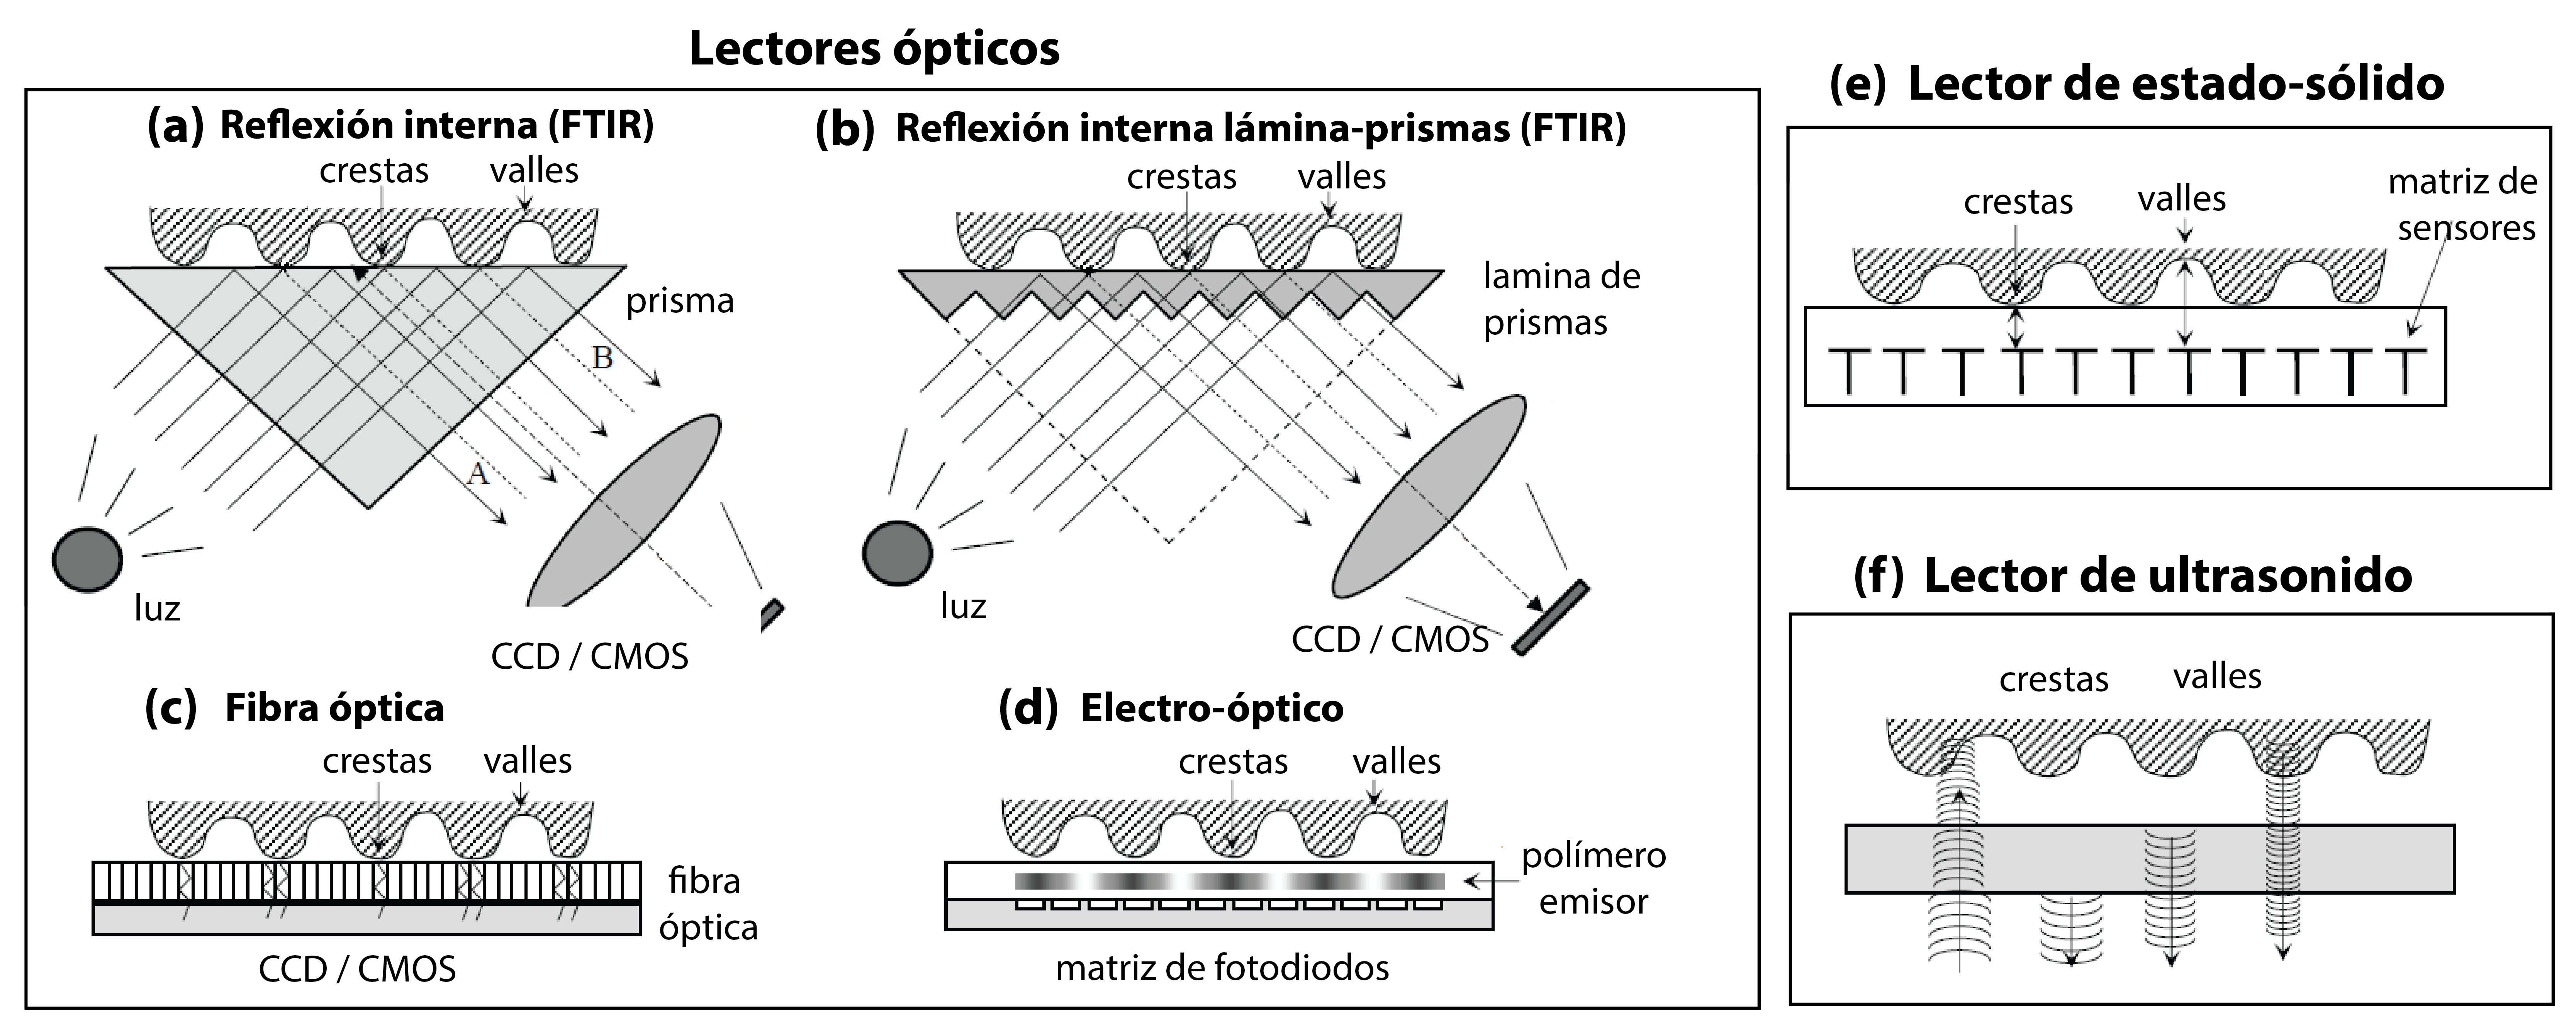
\includegraphics[width=1\linewidth]{ch-sistemasABC/images/ch-biometricosABC/sensores_dactilares.png}
    \caption{Tipos de lectores de huellas \cite{maltoni2009handbook}.}
    \label{fig:SensoresDactilares}
\end{figure}

El sensor debe tener una \textbf{resolución mínima de $500$ \gls{DPI}}.

Es recomendable usar lectores de huellas con mecanismos que eviten \textbf{fallos de lectura} por las condiciones de la piel. Por ejemplo, si la huella o el sensor tienen algo de \textbf{humedad}, la captura suele resultar demasiado oscura para extraer las características o también, si hay una diferencia de temperatura entre el dedo y el sensor, se genera un artefacto conocido como \textbf{<<halo>>} que dificulta la lectura. 
 
Mantener el \textbf{sensor limpio}, limpiándolo cuidadosamente, sin dañarlo y siguiendo las instrucciones del fabricante.

Los sensores no suelen realizar bien la captura cuando reciben una luz directa, producen un efecto similar al contraluz en al \gls{biometria} \gls{facial}, por ello, es conveniente \textbf{cubrir el sensor}. Esto también protege el sensor de otros factores ambiénteles, como la suciedad. 

Es importante tener en cuenta el \textbf{ángulo} y la \textbf{posición} del sensor. Al viajero le resulta más fácil colocar el \textbf{dedo índice} que el resto de los dedos. Y también, suele resultar mas cómodo usar la \textbf{mano derecha} que la izquierda.

También hay que tener el cuenta el \textbf{tamaño} del sensor si está cubierto, para que cualquier viajero pueda introducir la mano. 

Se puede pensar en usar \textbf{lectores móviles} para facilitar el proceso a personas con alguna discapacidad.


%%%%%%%%%%%%%%%%%%%%%%%%%%%%%%%%%%%%  ABC_BIOMETRICO:VERIFICACION DACTILAR EN ABC %%%%%%%%%%%%%%%%%%%%%%
\subsubsection{Verificación en la biometría dactilar}\label{subsec:VerificacionDactilarABC}

La verificación \gls{dactilar} consiste en comparar las características extraídas de la \textbf{huella capturada} con las características de la \textbf{huella pre-registrada} o las de la \textbf{huella del \gls{eMRTD}}. Por eso es importante que el sensor empleado para adquirir los tres rasgos tenga las \textbf{mismas especificaciones}\footnote{\GLS{ISO}/\GLS{IEC} $19794$-$4$:$2011$ \cite{ISO/Finger}, \GLS{EBTS} \cite{FBIBioOnline} y \GLS{BSI} TR-$03121$ \cite{BSI-TR-03121} proponen una serie de especificaciones y estándares para los lectores de huellas dactilares a la que deben atenerse todos los fabricantes dispositivos \GLS{ABC}.} para que se posible extraer las \textbf{mismas características}.

Es recomendable un \textbf{análisis de calidad} de la huella antes de proceder a la verificación ya que es una biometría en la que el usuario no tolera bien los \GLS{FRR}. 

El rendimiento del verificador deber ser al menos de un \textbf{\GLS{FAR}} del $0,1$\% y comprobar que para ese \GLS{FAR} el \textbf{\GLS{FRR}} no debe superar el $3$\%. 

Si se han registrado las \textbf{huellas de todos los dedos}, el sistema puede realizar también, la lectura de todos los dedos de una mano y elegir la huella leída con más calidad para minimizar el \GLS{FRR}, o solicitar una huella especifica, implementando una estrategia \textit{\gls{challenge response}} de \textbf{\textit{\gls{liveness detection}}}.   


%%%%%%%%%%%%%%%%%%%%%%%%%%%%%%%%%%%%  ABC_BIOMETRICO:BIOMETRIA DEL IRIS EN ABC %%%%%%%%%%%%%%%%%%%%%%
\section{Biometría del iris en los ABC}\label{sec:BiometriaIrisABC}

El \gls{iris} un rasgo biométrico también opcional, como la huella dactilar, en la segunda generación de \textit{\gls{e-passport}}\footnote{\GLS{ISO}/\GLS{EIC} $19794$-$6$ \cite{ISO/Iris} propone un estándar para las imágenes del \gls{iris} en los sistemas biométricos.} propuestos en \GLS{ICAO} doc 9309 \cite{doc20069303}.  

No es una \gls{biometria} muy aceptada debido a que resulta más intrusiva que la huella dactilar o la cara. Además, tiene algunos problemas, especialícenme en su adquisición, por razones de mala iluminación, parpadeo o movimiento involuntario de los ojos, que penalizan su rendimiento al verificar. 

\color{red} También hay sistemas que tratan de procesar el \gls{iris} en movimiento \cite{matey2006iris}. \color{black}

En la biometría del \gls{iris}, como en la \gls{facial}, la pose también puede ser un problema que penalice el rendimiento del sistema por lo algunos estudios tratan de darle una solución \cite{chou2009non}. 

La adquisición del \gls{iris} es similar a la adquisición en la biométrica facial por lo que es conveniente seguir las mismas recomendaciones que se exponen en el punto \ref{subsec:AdquisicionFacialABC}. Pero también hay algunas \textbf{recomendaciones especificas} para la biometría del \gls{iris}.

La \textbf{iluminación} afecta mucho en la captura del \gls{iris} ya que demasiada luz, puede hacer que la pupila se dilate y no sea posible leer la zona de textura del \gls{iris}.

La \textbf{distancia del viajero al sensor} debe estar más controlada, entre $80$ y $120$ cm, para poder conseguir imágenes de calidad, el estándar \GLS{ISO}/\GLS{EIC} $19794$-$6$ \cite{ISO/Iris}, recomienda una \textbf{resolución mínima} de $10$ píxeles por milímetro.  

Las gafas de sol no están permitidas en los sistemas \GLS{ABC}, pero la \gls{biometria} del \gls{iris} es más estricta y necesita que los cristales sean \textbf{completamente trasparentes} e incluso que \textbf{no provoquen reflejos}. 

Al viajero se le deben dar mensajes con \textbf{instrucciones más específicas}. Por ejemplo: Acercarse o alejarse, abrir más los ojos, retirarse las gafas o las lentes de contacto. 

Debe tener un rendimiento de al menos un \textbf{\GLS{FAR}} del $0,01$\% y para ese \GLS{FAR} el \textbf{\GLS{FRR}} no debe superar el $1$\%. 

\color{red}

IRIS RECOGNITION AT AIRPORT AND BORDER CROSSING ENCICLOPEDIA OF BIOMETRIC 

\GLS{ICAO} establece el iris como rasgo biométrico opcional para los \gls{e-passport}.

El $8$\% de los sistemas \GLS{ABC} en \GLS{EU} usan la biometria del iris para la verificación del viajero.

Los componentes principales de un sistema de \gls{biometria} de \gls{iris} son:

\begin{itemize}
    \item 
    Cámara de alta resolución que debe colocarse a distancia apropiada del viajero. Unos $25$cm si solo se requiere la adquisición de un ojo y a uno $100$cm si se requieren los dos ojos. Normamente ademas de una camara en el espctro visible, se requiere de una cámara \GLS{IR}.

    \item
    El sistema de iluminación suele requerir una luz en el infrarrojo cercano para evitar la influencia de la luz exterior.
    
    \item
    El módulo de verificación realiza la comparación entre la imagen del iris capturado y la imagen almacenada en los documentos o en la base de datos, dependiendo del sistema \GLS{ABC}. El algoritmo mas habitual para la comparación es el presentado en los estudios \cite{daugman2009iris} \cite{daugman2015iris}.

\end{itemize}

Los pasos a seguir en un sistema con \gls{biometria} del \gls{iris} son:

\begin{enumerate}
    \item 
    Indicar al viajero la pose.
    
    \item
    El sistema de iluminación controla sirve para controlar la posición del iris y la apertura de la pupila. Mediante un pulso de luz infrarroja se controla la dilatación de pupila para que aplicar la región del iris y que resulte mas fácil su captura.
    
    \item
    Se verifica la imagen capturada del iris con la almacenada en la documentación o la base de datos, dependiendo del tipo de sistema. 
\end{enumerate}

Los principales retos en la \gls{biometria} del \gls{iris} \cite{palmer2012ten}:

\begin{itemize}
    \item 
    Los sistemas de \gls{biometria} del \gls{iris} son más caros que otros sistemas biométricos.
    
    \item
    Aun o no están bien integrados con los sistemas externos. No todos los países almacenan información sobre el iris.
    
    \item
    Algunos viajeros consideran la \gls{biometria} del \gls{iris} como demasiado intrusiva. Es necesario desarrollar un métodos que simplifique la adquisición.
\end{itemize}

\color{black}


